\documentclass[11pt,a4paper,oneside]{book}

% ============================================================
% Encoding, typography, and page layout
% ============================================================
\usepackage[T1]{fontenc}
\usepackage[utf8]{inputenc}
\usepackage{newtxtext}
\usepackage[
  a4paper,
  top=2.45cm,
  bottom=2.55cm,
  inner=2.65cm,
  outer=2.45cm,
  headheight=22pt,
  headsep=0.48cm,
  footskip=0.95cm
]{geometry}
\usepackage{microtype}
\usepackage{parskip}
\usepackage{needspace}
\usepackage{setspace}

% ============================================================
% Mathematics
% ============================================================
\usepackage{amsmath}
\usepackage{amssymb}
\usepackage{mathtools}
\usepackage{newtxmath}

% ============================================================
% Tables and lists
% ============================================================
\usepackage{booktabs}
\usepackage{tabularx}
\usepackage{array}
\usepackage{longtable}
\usepackage{multirow}
\usepackage{enumitem}
\usepackage{listings}

% ============================================================
% Graphics
% ============================================================
\usepackage{graphicx}
% TikZ loads xcolor: enable table colours before that first load.
\usepackage[table]{xcolor}
\usepackage{tikz}
\usetikzlibrary{
  arrows.meta,
  positioning,
  fit,
  calc,
  shapes.geometric,
  backgrounds
}
\usepackage{pgfplots}
\pgfplotsset{compat=1.18}

% ============================================================
% Colour, boxes, headings, captions, navigation
% ============================================================
\usepackage[skins,breakable]{tcolorbox}
\usepackage{titlesec}
\usepackage{caption}
\usepackage{fancyhdr}
\usepackage{hyperref}
\usepackage[nameinlink,noabbrev]{cleveref}

% ============================================================
% Palette
% ============================================================
\definecolor{SapienzaRed}{RGB}{148,28,50}
\definecolor{AccentDark}{RGB}{116,22,40}
\definecolor{RemarkGray}{RGB}{72,72,76}
\definecolor{LineGray}{RGB}{183,183,188}
\definecolor{SoftRed}{RGB}{251,246,247}
\definecolor{SoftBlueGray}{RGB}{244,248,252}
\definecolor{SoftGreen}{RGB}{244,250,246}
\definecolor{SoftGray}{RGB}{247,247,248}
\definecolor{TableTint}{RGB}{249,241,243}
\definecolor{ClientBlue}{RGB}{242,248,253}
\definecolor{DataGreen}{RGB}{242,249,244}
\definecolor{MetaRed}{RGB}{251,244,246}
\definecolor{MapBlue}{RGB}{242,248,253}
\definecolor{ReduceGreen}{RGB}{242,249,244}
\definecolor{ShuffleTint}{RGB}{250,244,246}
\definecolor{DeepGreen}{RGB}{58,104,78}
\definecolor{LinkColor}{RGB}{112,22,40}
\definecolor{MutedBlue}{RGB}{63,108,142}
\definecolor{MutedGreen}{RGB}{79,122,98}
\definecolor{SoftCode}{RGB}{248,248,249}

% ============================================================
% General typography
% ============================================================
\setlength{\parindent}{0pt}
\setlength{\parskip}{0.50em}
\linespread{1.045}
\setlength{\emergencystretch}{2em}
\renewcommand{\arraystretch}{1.18}
\setcounter{tocdepth}{2}
\raggedbottom

\setlist[itemize]{leftmargin=1.55em,itemsep=0.22em,topsep=0.30em}
\setlist[enumerate]{leftmargin=1.80em,itemsep=0.25em,topsep=0.32em}

% ============================================================
% Chapter / section hierarchy
% ============================================================
\titleformat{\chapter}[display]
  {\normalfont\bfseries}
  {\color{SapienzaRed}\large\MakeUppercase{\chaptername}\ \thechapter}
  {0.45em}
  {\Huge}
  [\vspace{0.35em}\color{SapienzaRed}\titlerule]
\titlespacing*{\chapter}{0pt}{-0.45cm}{1.15cm}

\titleformat{\section}
  {\normalfont\Large\bfseries\color{SapienzaRed}}
  {\thesection}{0.72em}{}
\titleformat{\subsection}
  {\normalfont\large\bfseries}
  {\thesubsection}{0.66em}{}
\titleformat{\subsubsection}
  {\normalfont\normalsize\bfseries}
  {\thesubsubsection}{0.60em}{}

\titlespacing*{\section}{0pt}{1.40em}{0.60em}
\titlespacing*{\subsection}{0pt}{1.05em}{0.40em}
\titlespacing*{\subsubsection}{0pt}{0.90em}{0.32em}

% ============================================================
% Hyperlinks
% ============================================================
\hypersetup{
  colorlinks=true,
  linkcolor=LinkColor,
  urlcolor=LinkColor,
  citecolor=LinkColor,
  pdfauthor={Matt Clifford Trinidad Ramos},
  pdftitle={Big Data Computing -- Scale-Out Storage, MapReduce, and Apache Spark},
  pdfsubject={Big Data Infrastructure course notes},
  pdfkeywords={Big Data Computing, distributed storage, GFS, HDFS, MapReduce, Apache Spark, RDD, DAG}
}
\urlstyle{same}

% ============================================================
% Dynamic header and footer
% ============================================================
\pagestyle{fancy}
\fancyhf{}
\renewcommand{\chaptermark}[1]{\markboth{\thechapter.\ #1}{}}
\renewcommand{\sectionmark}[1]{\markright{\thesection.\ #1}}
\fancyhead[L]{\small\nouppercase{\leftmark}}
\fancyhead[R]{\small\nouppercase{\rightmark}}
\fancyfoot[L]{\small Big Data Computing}
\fancyfoot[C]{\small \thepage}
\fancyfoot[R]{\small Matt Clifford Trinidad Ramos}
\renewcommand{\headrulewidth}{0.45pt}
\renewcommand{\footrulewidth}{0.45pt}
\renewcommand{\headrule}{\hbox to\headwidth{\color{SapienzaRed}\leaders\hrule height \headrulewidth\hfill}}
\renewcommand{\footrule}{\hbox to\headwidth{\color{SapienzaRed}\leaders\hrule height \footrulewidth\hfill}}

\fancypagestyle{plain}{
  \fancyhf{}
  \fancyfoot[L]{\small Big Data Computing}
  \fancyfoot[C]{\small \thepage}
  \fancyfoot[R]{\small Matt Clifford Trinidad Ramos}
  \renewcommand{\headrulewidth}{0pt}
  \renewcommand{\footrulewidth}{0.45pt}
  \renewcommand{\footrule}{\hbox to\headwidth{\color{SapienzaRed}\leaders\hrule height \footrulewidth\hfill}}
}

% ============================================================
% Selective semantic boxes
% ============================================================
\tcbset{
  academicbox/.style={
    enhanced,breakable,
    boxrule=0.55pt,arc=0.8mm,
    left=2.2mm,right=2.2mm,top=1.6mm,bottom=1.6mm,
    before skip=0.75em,after skip=0.75em
  }
}

\newtcolorbox{keyconcept}{
  academicbox,
  colback=SoftRed,colframe=SapienzaRed,
  colbacktitle=SoftRed,coltitle=SapienzaRed,
  title={Key Concept},fonttitle=\bfseries,
  borderline west={1.6pt}{0pt}{SapienzaRed}
}

\newtcolorbox{definitionbox}[1]{
  academicbox,
  colback=SoftRed,colframe=SapienzaRed,
  colbacktitle=SapienzaRed,coltitle=white,
  title={Definition -- #1},fonttitle=\bfseries
}

\newtcolorbox{remarkbox}[1]{
  academicbox,
  colback=SoftGray,colframe=LineGray,
  colbacktitle=SoftGray,coltitle=RemarkGray,
  title={Remark -- #1},fonttitle=\bfseries,
  borderline west={1.4pt}{0pt}{RemarkGray}
}

\newtcolorbox{examplebox}[1]{
  academicbox,
  colback=SoftRed,colframe=SapienzaRed,
  colbacktitle=white,coltitle=SapienzaRed,
  title={Example -- #1},fonttitle=\bfseries,
  borderline west={1.4pt}{0pt}{SapienzaRed}
}

% ============================================================
% Captions and reusable TikZ styles
% ============================================================
\captionsetup{font=small,labelfont={bf,color=SapienzaRed},justification=justified,singlelinecheck=false}

\tikzset{
  metadata/.style={draw=SapienzaRed,fill=MetaRed,rounded corners=1.2mm,minimum height=9mm,minimum width=2.8cm,align=center,font=\small},
  datanode/.style={draw=DeepGreen,fill=DataGreen,rounded corners=1.2mm,minimum height=9mm,minimum width=2.7cm,align=center,font=\small},
  clientnode/.style={draw=RemarkGray,fill=ClientBlue,rounded corners=1.2mm,minimum height=9mm,minimum width=2.5cm,align=center,font=\small},
  control/.style={-{Latex[length=2mm]},dashed,thick,draw=RemarkGray},
  dataflow/.style={-{Latex[length=2.2mm]},very thick,draw=DeepGreen},
  controlbi/.style={{Latex[length=2mm]}-{Latex[length=2mm]},dashed,thick,draw=RemarkGray},
  storagenode/.style={draw=RemarkGray,fill=SoftGray,rounded corners=1.2mm,minimum height=8mm,minimum width=2.4cm,align=center,font=\small},
  mapnode/.style={draw=RemarkGray,fill=MapBlue,rounded corners=1.2mm,minimum height=8mm,minimum width=2.25cm,align=center,font=\small},
  reducernode/.style={draw=DeepGreen,fill=ReduceGreen,rounded corners=1.2mm,minimum height=8mm,minimum width=2.35cm,align=center,font=\small},
  masternode/.style={draw=SapienzaRed,fill=SoftRed,rounded corners=1.2mm,minimum height=8mm,minimum width=2.7cm,align=center,font=\small},
  datarrow/.style={-{Latex[length=2mm]},thick,draw=DeepGreen},
  ctrlarrow/.style={-{Latex[length=2mm]},dashed,thick,draw=RemarkGray},
  shufflearrow/.style={-{Latex[length=2mm]},thick,draw=SapienzaRed}
}

\newcolumntype{Y}{>{\raggedright\arraybackslash}X}
\newcolumntype{C}[1]{>{\centering\arraybackslash}p{#1}}

% ============================================================
% Code snippets
% ============================================================
\lstdefinestyle{sparkcode}{
  language=Python,
  basicstyle=\ttfamily\small,
  backgroundcolor=\color{SoftCode},
  frame=single,
  rulecolor=\color{LineGray},
  framesep=4pt,
  xleftmargin=0.8em,
  xrightmargin=0.8em,
  aboveskip=0.75em,
  belowskip=0.75em,
  showstringspaces=false,
  columns=fullflexible,
  keepspaces=true,
  breaklines=true,
  breakatwhitespace=true,
  tabsize=2,
  commentstyle=\itshape\color{RemarkGray},
  keywordstyle=\bfseries\color{SapienzaRed},
  stringstyle=\color{MutedBlue}
}

\begin{document}

% ============================================================
% Title page
% ============================================================
\hypersetup{pageanchor=false}
\begin{titlepage}
\thispagestyle{empty}
\centering
\vspace*{0.5cm}

% Official logo: https://www.uniroma1.it/it/pagina/impaginazione-della-tesi-e-logo
\IfFileExists{assets/sapienza-logo.png}{%
  \noindent\makebox[\textwidth][l]{
\includegraphics[width=7.5cm]{assets/sapienza-logo.png}}\par
}{%
  \noindent\makebox[\textwidth][l]{%
    \begin{minipage}{7.5cm}
      {\color{SapienzaRed}\Large\bfseries SAPIENZA}\par
      {\small UNIVERSIT\`A DI ROMA}
    \end{minipage}}
  \par
}
\vspace{1.0cm}

{\color{SapienzaRed}\rule{0.84\textwidth}{0.9pt}}
\vspace{0.78cm}

{\LARGE\bfseries\MakeUppercase{Big Data Computing}\par}
\vspace{0.32cm}
{\Large Course Notes\par}
\vspace{0.52cm}
{\normalsize Academic Year 2026/2027\par}

\vspace{0.78cm}
{\color{SapienzaRed}\rule{0.84\textwidth}{0.9pt}}

\vfill

{\small\textsc{Lecturer}\par}
\vspace{0.12cm}
{\large Gabriele Tolomei\par}

\vspace{0.70cm}
{\small Department of Computer Science\par}
{\small Sapienza University of Rome\par}

\vspace{1.25cm}

{\small\textsc{Notes prepared by}\par}
\vspace{0.12cm}
{\large\bfseries Matt Clifford Trinidad Ramos\par}

\vfill
\end{titlepage}

\frontmatter
\hypersetup{pageanchor=true}
\tableofcontents

\chapter*{Course Information}
\addcontentsline{toc}{chapter}{Course Information}
\markboth{Course Information}{Course Information}

\begin{table}[htbp]
\centering
\caption*{Course at a glance}
\begin{tabularx}{\textwidth}{>{\bfseries\raggedright\arraybackslash}p{3.5cm} Y}
\toprule
Course & Big Data Computing, M.Sc. in Computer Science \\
Academic year & 2026/2027 \\
Lecturer & Gabriele Tolomei \\
Class schedule & Wednesday 08:00--11:00 (Room 1L); Thursday 10:00--12:00 (Room 2L) \\
Office & Room 106, first floor, Building E, Viale Regina Elena 295 \\
Course website & \url{https://gtolomei.github.io/teaching/bdc.html} \\
\bottomrule
\end{tabularx}
\end{table}

\section*{Assessment}
The final grade is based on an oral seminar about a recent, high-impact research paper selected by the student and approved by the instructor. The course material identifies top-tier venues such as SIGMOD, VLDB, OSDI, SOSP, NeurIPS, ICML, and KDD as representative sources.

\begin{table}[htbp]
\centering
\caption*{Seminar format}
\begin{tabular}{lccc}
\toprule
\rowcolor{TableTint}
Format & Presentation & Q\&A & Total \\
\midrule
Individual & $\sim$12 min & $\sim$3 min & $\sim$15 min \\
Pair & $\sim$25 min & $\sim$5 min & $\sim$30 min \\
\bottomrule
\end{tabular}
\end{table}

For pair presentations, presentation time and Q\&A should be balanced between the two students. The course material states that honors (30 cum laude) require exceptional mastery of the topic, deep critical insight, and flawless academic communication.

\section*{Course Organization}
{\small
\begin{itemize}[leftmargin=1.4em,itemsep=0.08em,topsep=0.18em]
  \item \textbf{Big Data Infrastructure:} scale-out storage, MapReduce, Spark/DAG execution, streaming, and fault tolerance.
  \item \textbf{High-Dimensional Data Representations:} high-dimensional geometry, Johnson--Lindenstrauss reduction, columnar layouts, and embeddings.
  \item \textbf{Classical Non-Learning Tasks:} indexing, sampling, Approximate Query Processing, sketches (HyperLogLog, Count-Min), and Locality-Sensitive Hashing.
  \item \textbf{Scale-Out Learning Systems:} large-scale ERM, parallel/asynchronous SGD, Parameter Server, Federated Learning, and memory-bandwidth optimization.
\end{itemize}

\textbf{Suggested references.} Leskovec, Rajaraman, and Ullman, \emph{Mining of Massive Datasets}; Blum, Hopcroft, and Kannan, \emph{Foundations of Data Science}; Kleppmann, \emph{Designing Data-Intensive Applications}; Manning, Raghavan, and Schütze, \emph{Introduction to Information Retrieval}; Shalev-Shwartz and Ben-David, \emph{Understanding Machine Learning}; plus research papers referenced throughout the course material.
}

\clearpage
\mainmatter

\chapter[Scale-Out Paradigm and Distributed Storage]{Scale-Out Paradigm and Distributed\\Storage}
\label{chap:scale-out-storage}

A single machine is constrained by finite processor, memory, storage, network, power, and cooling resources. Big data infrastructure therefore replaces the assumption of one sufficiently large and reliable machine with a cluster of cooperating machines whose aggregate capacity can grow over time. This change in scale also changes the failure model: individual disks, nodes, and network components are expected to fail while the overall system continues to operate.

Distributed storage provides the substrate for this model. Large files are divided into independently managed blocks or chunks, metadata is separated from bulk data transfer, and replicas are placed across machines and racks so that data remains available after ordinary failures. Google File System (GFS) and Hadoop Distributed File System (HDFS) instantiate these principles and expose the physical placement information later used by distributed computation frameworks.

\begin{keyconcept}
At scale, reliability is a property of the distributed software rather than of any individual machine. Commodity components may fail; the system survives by detecting those failures, maintaining redundant data, and reconstructing lost replicas automatically.
\end{keyconcept}

\section{Why Scale Out?}
% ============================================================

\subsection{The Data Growth Problem}

Data growth can outpace the capacity growth of an individual machine. Increasing the capacity of one disk or one server every few years does not solve workloads whose data volume grows on a much shorter timescale. Representative examples include web crawls containing hundreds of billions of pages and petabytes of raw HTML, telemetry and clickstream data accumulating at terabytes per day, and scientific or enterprise datasets that can reach exabyte scale.

\begin{figure}[htbp]
\centering
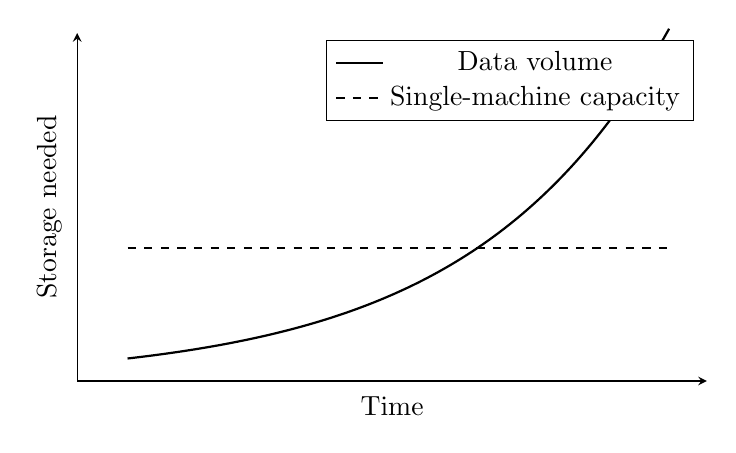
\begin{tikzpicture}
\begin{axis}[
  width=0.79\textwidth,
  height=6.0cm,
  axis lines=left,
  xlabel={Time},
  ylabel={Storage needed},
  xmin=0,xmax=10,
  ymin=0,ymax=11,
  xtick=\empty,
  ytick=\empty,
  clip=false
]
\addplot[thick,domain=0.8:9.4,samples=100] {0.55*exp(0.32*x)};
\addlegendentry{Data volume}
\addplot[thick,dashed,domain=0.8:9.4] {4.2};
\addlegendentry{Single-machine capacity}
\end{axis}
\end{tikzpicture}
\caption{Conceptual representation of the data-growth problem. The curves are schematic and do not encode measured experimental data.}
\label{fig:data-growth}
\end{figure}

Figure~\ref{fig:data-growth} captures the qualitative scaling argument: if demand grows faster than the capacity of an individual machine, periodically replacing that machine only moves the ceiling.

\subsection{Single-Machine Limits}

A powerful server still faces finite physical resources:

\begin{itemize}
    \item \textbf{CPU:} finite cores per socket and finite sockets per motherboard;
    \item \textbf{RAM:} finite DIMM slots and finite addressable memory;
    \item \textbf{Disk:} finite drive bays and finite controller bandwidth;
    \item \textbf{Network:} finite NIC bandwidth entering and leaving one machine.
\end{itemize}

These are hard ceilings. A larger machine may postpone the limit, but it does not remove the existence of a limit.

\subsection{Vertical Scaling}

\begin{definitionbox}{Vertical Scaling / Scale Up}
Vertical scaling means increasing the capacity of a single machine by adding or upgrading CPU cores, RAM, disks, and other resources within the same node.
\end{definitionbox}

Scale up is conceptually attractive because the software model often remains unchanged: the same machine simply has more resources. Its weakness appears at the high end, where price does not grow linearly with capacity.

\begin{table}[htbp]
\centering
\caption{Illustrative vertical-scaling cost curve.}
\label{tab:vertical-cost}
\begin{tabularx}{0.78\textwidth}{Y C{2.8cm} C{2.8cm}}
\toprule
\rowcolor{TableTint}
\textbf{Configuration} & \textbf{Relative capacity} & \textbf{Relative cost} \\
\midrule
Commodity server & $1\times$ & $1\times$ \\
High-end server & $4\times$ & $\sim 10\times+$ \\
Top-of-line mainframe-class & $16\times$ & $\sim 100\times+$ \\
\bottomrule
\end{tabularx}
\end{table}

Premium hardware introduces a steep price premium. Beyond cost, vertical scaling eventually reaches physical limits imposed by motherboard capacity, power, cooling, and machine design. Vertical scaling therefore buys time, but it does not provide a long-term strategy for web-scale or exabyte-scale workloads.

\subsection{Horizontal Scaling}

\begin{definitionbox}{Horizontal Scaling / Scale Out}
Horizontal scaling means increasing total system capacity by adding more independent machines to a cluster rather than making a single machine larger.
\end{definitionbox}

The workload is distributed over many relatively modest nodes. Capacity grows by adding nodes, which makes horizontal scaling the foundational strategy behind big data systems.

A key design philosophy in systems such as GFS and HDFS is to build clusters from inexpensive commodity machines rather than from a few premium, highly reliable servers. Individual node failure is expected. Reliability is therefore provided by the distributed software rather than entrusted entirely to the hardware.

\begin{keyconcept}
Scale-out infrastructure replaces the assumption of highly reliable individual hardware with software-level fault tolerance across many inexpensive components.
\end{keyconcept}

\subsection{Vertical versus Horizontal Scaling}

\begin{table}[htbp]
\centering
\caption{Comparison between vertical and horizontal scaling across the main design dimensions.}
\label{tab:scale-comparison}
\begin{tabularx}{\textwidth}{>{\bfseries\raggedright\arraybackslash}p{3.1cm} Y Y}
\toprule
\rowcolor{TableTint}
Aspect & Vertical (Scale Up) & Horizontal (Scale Out) \\
\midrule
Approach & Bigger single machine & More machines \\
Ceiling & Hard physical limit & Limited by coordination, network, and workload scalability \\
Cost growth & Superlinear at the high end & Roughly linear with commodity hardware \\
Failure handling & Hardware reliability & Software-level fault tolerance \\
Complexity & Lower; same software model & Higher; distributed coordination is required \\
\bottomrule
\end{tabularx}
\end{table}

The advantage of scale out is therefore not that distribution is simpler. It is that distribution avoids the hard capacity ceiling of one machine and allows the system to expand using commodity resources.

\subsection{The New Failure Model}

At cluster scale, hardware failure becomes a continuous background process. Disks fail, machines crash, network links become temporarily unavailable, and entire racks can lose power. A system designed under the assumption that failure is rare will encounter its ``rare'' cases continuously when deployed across thousands of components.

\subsection{Cost per Byte and Cost per FLOP}

Two economic dimensions become especially important at scale:

\begin{itemize}
    \item \textbf{Cost per byte:} commodity disks make raw storage inexpensive, so replication and durability overhead become important.
    \item \textbf{Cost per FLOP:} commodity CPUs make raw computation inexpensive, so coordination and data movement become important.
\end{itemize}

In both cases, the challenge shifts away from the unit price of hardware and toward the efficiency with which the system coordinates many cheap components.

\subsubsection*{Review Questions}
\begin{enumerate}
    \item What is the fundamental difference between vertical and horizontal scaling?
    \item Why does vertical scaling eventually hit a hard physical ceiling?
    \item Why do big data systems prefer many commodity machines over a few premium machines?
    \item Why must failure be treated as a normal event in scale-out systems?
\end{enumerate}


% ============================================================
\section{Foundations of Distributed Storage}
% ============================================================

\subsection{The Distributed File System Abstraction}

\begin{definitionbox}{Distributed File System}
A distributed file system (DFS) presents a unified file-system interface while the underlying data is physically distributed across many machines. Files appear as part of one logical namespace even though their contents are split into blocks, replicated, and stored on multiple servers.
\end{definitionbox}

The DFS hides physical distribution behind ordinary file operations such as open, read, write, and close. The design target is petabyte-scale storage that remains usable through a familiar file abstraction.

\subsection{Throughput versus Latency}

Big data DFSs are designed primarily for \emph{throughput}: the amount of data transferred per unit time across the cluster. They tolerate higher latency for individual operations because batch processing over very large datasets benefits more from aggregate bandwidth than from millisecond-scale response to isolated requests.

\begin{remarkbox}{Design target}
High latency is not itself desirable; the deliberate optimization target is aggregate throughput rather than minimum per-request latency for large batch workloads.
\end{remarkbox}

\subsection{Huge Files and Sequential Access}

The expected workload contains files ranging from gigabytes to terabytes and predominantly sequential access. Random small reads and writes are not the primary target. This assumption influences block size, metadata design, replication, and the write model.

\subsection{Write-Once, Read-Many}

A common lifecycle is that a file is written once, possibly through appends, then closed and read many times by analytical jobs. Arbitrary in-place updates are rare or disallowed. Relaxing support for random in-place modification removes a significant consistency and coordination burden.

\subsection{The Block / Chunk Abstraction}

\begin{definitionbox}{Block / Chunk}
A block or chunk is a storage unit with a configured maximum size into which a large file is divided; the final unit may be shorter. Blocks are stored, replicated, placed, and recovered independently, and different blocks of the same logical file may reside on different machines.
\end{definitionbox}

The fixed-size abstraction is one of the most important design decisions in distributed storage. It simplifies metadata, load balancing, replication, and later parallel computation.

\subsection{Why Fixed-Size Blocks?}

Tracking blocks rather than arbitrary byte ranges simplifies the metadata model. Uniform blocks are also easier to move and rebalance, and each block can be replicated independently using a uniform mechanism.

\begin{table}[htbp]
\centering
\caption{Block-size trade-offs in distributed storage.}
\label{tab:block-size}
\begin{tabularx}{\textwidth}{>{\bfseries\raggedright\arraybackslash}p{3.2cm} Y Y}
\toprule
\rowcolor{TableTint}
Block size & Advantages & Disadvantages \\
\midrule
Small (e.g.\ 4 KB) & Fine-grained placement; low waste for small files & Huge metadata overhead at scale \\
Large (e.g.\ 64--128 MB) & Low metadata overhead; efficient sequential I/O & Small-file metadata overhead; coarser load balancing \\
\bottomrule
\end{tabularx}
\end{table}

Big data DFSs therefore choose blocks that are orders of magnitude larger than conventional local file-system blocks. A small file does not reserve an entire large block on disk: the main small-file costs are metadata and limited parallelism.

\subsection{Metadata and Data Separation}

A central architectural decision is to separate information about \emph{where data is} from the \emph{actual bytes}. The metadata service tracks the namespace and file-to-block or block-to-location mappings; data servers store block contents on local disks.

This separation allows metadata lookup and bulk I/O to be optimized independently.

\begin{figure}[htbp]
\centering
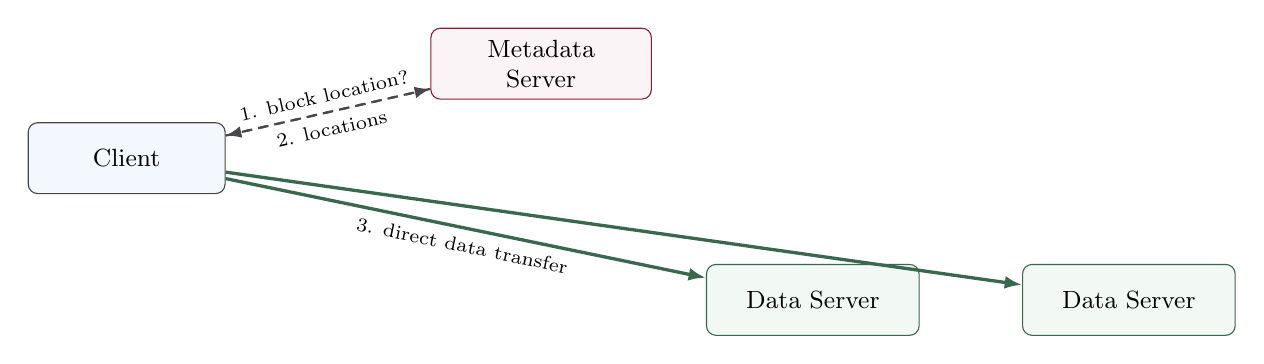
\begin{tikzpicture}[node distance=18mm and 26mm]
\node[clientnode] (client) {Client};
\node[metadata, right=of client, yshift=12mm] (meta) {Metadata\\Server};
\node[datanode, right=of client, yshift=-18mm, xshift=35mm] (data1) {Data Server};
\node[datanode, right=13mm of data1] (data2) {Data Server};

\draw[control] (client) -- node[above,sloped,font=\scriptsize]{1. block location?} (meta);
\draw[control] (meta) -- node[below,sloped,font=\scriptsize]{2. locations} (client);
\draw[dataflow] (client) -- node[below,sloped,font=\scriptsize]{3. direct data transfer} (data1);
\draw[dataflow] (client) -- (data2);
\end{tikzpicture}
\caption{Generic DFS interaction model. Metadata is obtained from a coordinator, while bulk data transfer occurs directly between the client and data servers.}
\label{fig:generic-dfs}
\end{figure}

The metadata server is deliberately removed from the large data path. This avoids turning the coordinator into a bandwidth bottleneck.

\subsection{Single Point of Coordination}

A single metadata coordinator offers a globally consistent namespace view and avoids distributed consensus for every metadata update. The trade-off is equally direct: the coordinator may become both a single point of failure and a scalability bottleneck.

\subsection{Namespace Management}

The metadata service maintains the directory hierarchy, the mapping from files to blocks, and the mapping from blocks to replicas. This metadata is kept primarily in memory to support fast lookups.

\subsection{Network Topology Awareness}

Clusters are physically hierarchical. Machines belong to racks, racks are connected by switches, and communication within a rack is typically less costly than communication across racks. Placement and scheduling therefore consider physical topology rather than treating every machine as equally distant.

\subsection{Why Replication Is Necessary}

RAID can protect against some disk failures inside one machine, but it cannot protect against the loss of the entire node, rack, or network path. Distributed storage therefore replicates data across machines and, ideally, across racks.

\begin{keyconcept}
Replication is not merely a performance optimization in a scale-out DFS. It is a primary durability mechanism that allows the logical file system to survive ordinary hardware failures.
\end{keyconcept}

\subsubsection*{Review Questions}
\begin{enumerate}
    \item Why do big data DFSs use large block sizes instead of small ones?
    \item Why is metadata kept separate from the actual data servers?
    \item In the client interaction model, what does the metadata server \emph{not} do?
    \item Why is RAID-style protection insufficient at cluster scale?
\end{enumerate}


% ============================================================
\section{The Google File System (GFS)}
% ============================================================

\subsection{Motivation and Original Context}

The Google File System (GFS), published in 2003, was designed for Google's internal workloads: large web crawls, logs, and index files stored on thousands of commodity machines. It assumes frequent component failures, huge files, sequential reads, and append-heavy writes rather than general-purpose POSIX semantics.

GFS later became the direct architectural inspiration for HDFS.

\subsection{Architecture Overview}

GFS uses one Master for metadata and many Chunkservers for actual data.

\begin{figure}[htbp]
\centering
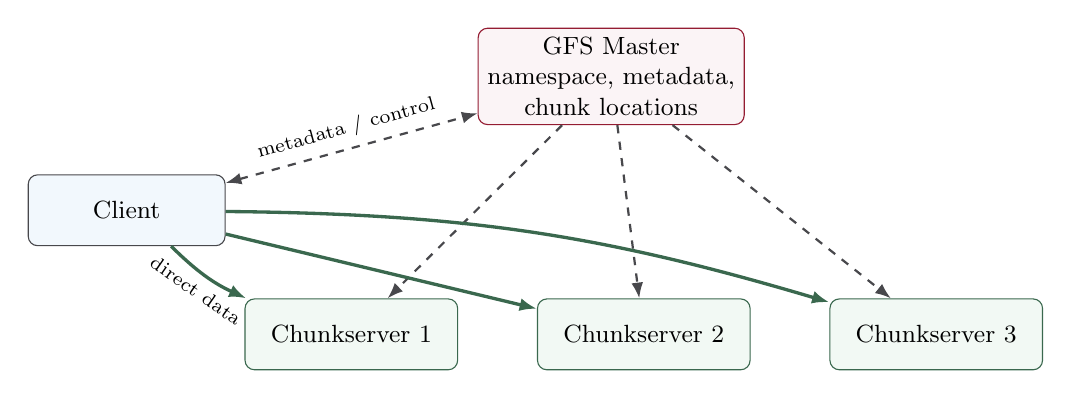
\begin{tikzpicture}[node distance=15mm and 15mm]
\node[clientnode] (client) {Client};
\node[metadata, right=32mm of client, yshift=17mm] (master) {GFS Master\\namespace, metadata,\\chunk locations};
\node[datanode, below=22mm of master, xshift=-33mm] (cs1) {Chunkserver 1};
\node[datanode, right=10mm of cs1] (cs2) {Chunkserver 2};
\node[datanode, right=10mm of cs2] (cs3) {Chunkserver 3};

\draw[controlbi] (client) -- node[above,sloped,font=\scriptsize]{metadata / control} (master);
\draw[control] (master) -- (cs1);
\draw[control] (master) -- (cs2);
\draw[control] (master) -- (cs3);

\draw[dataflow] (client) to[bend right=10] node[below,sloped,font=\scriptsize]{direct data} (cs1);
\draw[dataflow] (client) -- (cs2);
\draw[dataflow] (client) to[bend left=8] (cs3);
\end{tikzpicture}
\caption{GFS architecture. The Master coordinates metadata, while Chunkservers store and serve the actual chunk data directly to clients.}
\label{fig:gfs-architecture}
\end{figure}

\subsection{The GFS Master}

The Master is the single metadata-managing node. It maintains:

\begin{itemize}
    \item the file-system namespace;
    \item file-to-chunk mappings;
    \item chunk-to-Chunkserver locations;
    \item chunk lease assignments;
    \item coordination of chunk creation, replication, deletion, and garbage collection.
\end{itemize}

Master metadata is kept in memory for speed. Chunk-location information is not persisted in the same way as namespace mutations; it can be reconstructed by polling Chunkservers at startup.

The trade-off is that the namespace is bounded by the amount of Master memory.

\subsection{Why a Single Master?}

The design deliberately avoids a distributed metadata cluster. One Master greatly simplifies global decisions and avoids consensus on every metadata mutation. The risks are a potential bottleneck and a potential single point of failure, both of which require explicit mitigation.

\subsection{Chunkservers}

Chunkservers store GFS chunks as regular files on their local Linux file systems. They serve chunk reads and writes directly to clients and periodically report their state and chunk inventories to the Master.

\subsection{Chunk Size}

GFS uses 64 MB chunks. Large chunks reduce the number of chunks per file, decrease Master metadata, reduce client--Master lookup frequency, and encourage sustained sequential transfer. The accepted disadvantage is inefficiency for small files.

\subsection{Replication Factor}

The default replication factor is three. Replicas are placed on different Chunkservers with rack awareness, and the replication factor may be adjusted per file.

\subsection{Master--Chunkserver Heartbeats}

Heartbeats allow Chunkservers to report liveness, status, and chunk inventory. The Master can piggyback commands, such as replicate or delete, on heartbeat responses.

\begin{figure}[htbp]
\centering
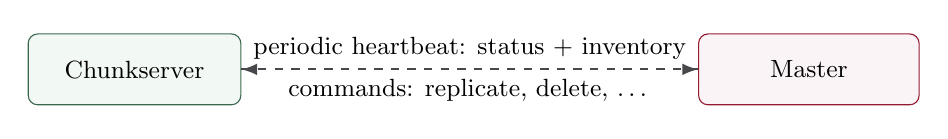
\begin{tikzpicture}[node distance=58mm]
\node[datanode] (cs) {Chunkserver};
\node[metadata, right=of cs] (m) {Master};

\draw[control] (cs) -- node[above,font=\small]{periodic heartbeat: status + inventory} (m);
\draw[control] (m) -- node[below,font=\small]{commands: replicate, delete, \ldots} (cs);
\end{tikzpicture}
\caption{Master--Chunkserver heartbeat interaction in GFS.}
\label{fig:gfs-heartbeat}
\end{figure}

\subsection{GFS Read Path}

For a read, the client first determines which chunk contains the requested file offset, obtains the chunk handle and replica locations from the Master, then communicates directly with a suitable Chunkserver.

\begin{enumerate}
    \item The client computes the chunk index for the requested file offset.
    \item The client asks the Master for the chunk handle and Chunkserver locations.
    \item The Master returns the handle and the locations; the client may cache them briefly.
    \item The client contacts the nearest replica directly.
    \item The Chunkserver streams the data directly to the client.
\end{enumerate}

\begin{figure}[htbp]
\centering
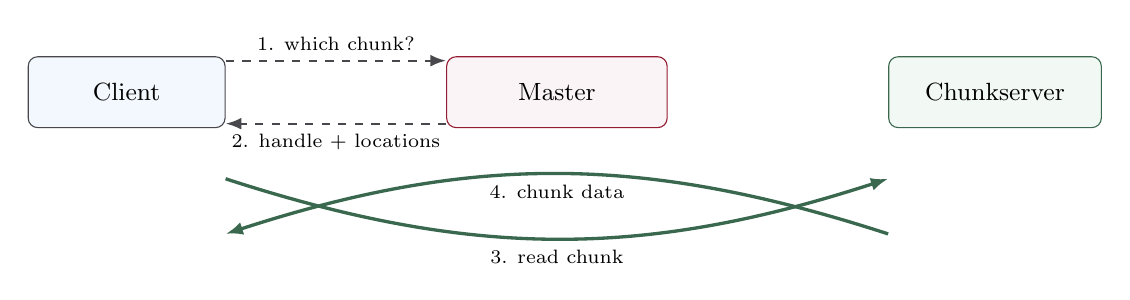
\begin{tikzpicture}[node distance=28mm]
\node[clientnode] (c) {Client};
\node[metadata, right=of c] (m) {Master};
\node[datanode, right=of m] (s) {Chunkserver};

\draw[control] ([yshift=4mm]c.east) -- node[above,font=\scriptsize]{1. which chunk?} ([yshift=4mm]m.west);
\draw[control] ([yshift=-4mm]m.west) -- node[below,font=\scriptsize]{2. handle + locations} ([yshift=-4mm]c.east);

\draw[dataflow] ([yshift=-11mm]c.east) to[bend right=18] node[below,font=\scriptsize]{3. read chunk} ([yshift=-11mm]s.west);
\draw[dataflow] ([yshift=-18mm]s.west) to[bend right=18] node[below,font=\scriptsize]{4. chunk data} ([yshift=-18mm]c.east);
\end{tikzpicture}
\caption{GFS read path. The Master supplies metadata; bulk data bypasses the Master and flows directly between the client and a Chunkserver.}
\label{fig:gfs-read}
\end{figure}

\begin{keyconcept}
The Master is on the metadata path, not on the bulk-data path. This separation keeps the metadata coordinator from becoming a data-transfer bottleneck.
\end{keyconcept}

\subsection{GFS Write Path}

GFS separates the transfer of bytes from the ordering of mutations. The original GFS design pipelines the data through a chain of replicas chosen to exploit network proximity; the primary is special for \emph{control and ordering}, not because all data must pass through it.

\begin{enumerate}
    \item The client asks the Master which Chunkservers hold the replicas and which replica currently holds the lease.
    \item The client starts pushing the data to a nearby replica; the replicas forward the data along a carefully chosen chain until every replica has buffered it.
    \item After all replicas have received the data, the client sends the write request to the primary replica.
    \item The primary assigns a serial order to the mutation and forwards the ordered request to the secondary replicas.
    \item The secondaries apply the mutation and acknowledge the primary; the primary then acknowledges the client.
\end{enumerate}

\begin{figure}[htbp]
\centering
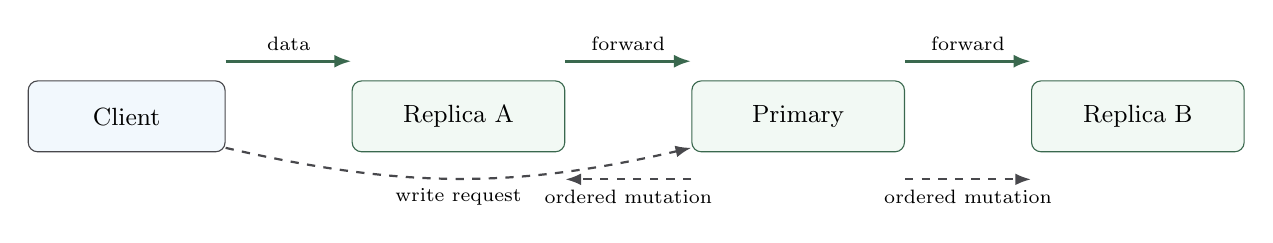
\begin{tikzpicture}[node distance=16mm]
\node[clientnode] (c) {Client};
\node[datanode, right=of c] (s1) {Replica A};
\node[datanode, right=of s1] (p) {Primary};
\node[datanode, right=of p] (s2) {Replica B};

% Pipelined data path.
\draw[dataflow] ([yshift=7mm]c.east) -- node[above,font=\scriptsize]{data} ([yshift=7mm]s1.west);
\draw[dataflow] ([yshift=7mm]s1.east) -- node[above,font=\scriptsize]{forward} ([yshift=7mm]p.west);
\draw[dataflow] ([yshift=7mm]p.east) -- node[above,font=\scriptsize]{forward} ([yshift=7mm]s2.west);

% Control path: client -> primary -> secondaries.
\draw[control] ([yshift=-4mm]c.east) to[bend right=13] node[below,font=\scriptsize]{write request} ([yshift=-4mm]p.west);
\draw[control] ([yshift=-8mm]p.west) -- node[below,font=\scriptsize]{ordered mutation} ([yshift=-8mm]s1.east);
\draw[control] ([yshift=-8mm]p.east) -- node[below,font=\scriptsize]{ordered mutation} ([yshift=-8mm]s2.west);
\end{tikzpicture}
\caption{GFS write control and data flow. Data is pipelined through replicas, while mutation ordering is controlled by the lease-holding primary.}
\label{fig:gfs-write}
\end{figure}

\begin{remarkbox}{Data flow versus control flow}
A simplified description often says that the client pushes data to all replicas. In the original GFS design, the replicas form a network-aware pipeline: the client initiates the transfer and each Chunkserver forwards data to the next. The conceptual point is unchanged: data movement is decoupled from the primary's ordering of mutations.
\end{remarkbox}

\subsection{Primary and Secondary Replicas}

The lease mechanism designates one replica as primary for a bounded period. The primary decides the serial order of concurrent mutations. Secondary replicas apply those mutations in the order dictated by the primary.

This delegates ordering to one replica rather than requiring the Master to order every write.

\subsection{Mutation Ordering and Consistency}

Successful writes use a common mutation order across replicas. Concurrent successful writes may leave a consistent but undefined region containing fragments of different writes; failed mutations can leave replicas inconsistent. Record append guarantees an atomic append at least once, so applications must handle possible duplicate records and padding. This is a relaxed consistency model rather than strict POSIX semantics.

\subsection{Chunk Leases}

The Master grants a time-bounded lease to a replica. The lease may be extended while the replica is actively handling mutations. If the primary becomes unreachable, a new lease can be granted after the old lease expires.

\subsection{Garbage Collection}

Deletion is lazy. A deleted file is renamed to a hidden name and retained for several days. Actual chunk storage is reclaimed later during normal Master--Chunkserver communication. This reduces synchronous cluster-wide deletion work and provides a short recovery window for accidental deletions.

\subsection{Operation Log and Checkpoints}

Namespace mutations are appended to a persistent operation log that is replicated to multiple machines. Periodically, the Master writes a compact checkpoint of its state. Recovery consists of loading the latest checkpoint and replaying subsequent log entries.

\subsection{Shadow Masters}

Shadow masters continuously apply the operation log and maintain read-only replicas of Master state. They can serve read-only metadata requests, but they do not automatically assume full write coordination after a primary Master failure.

\subsection{Limitations}

The original single-Master design introduces three major limitations:

\begin{itemize}
    \item the namespace must fit in one machine's memory;
    \item high metadata-operation rates can overload the Master;
    \item Master failover is not instantaneous.
\end{itemize}

These limitations motivate later HDFS mechanisms such as Federation and explicit high-availability configurations.

\subsubsection*{Review Questions}
\begin{enumerate}
    \item What two types of information does the GFS Master manage, and why is metadata kept in memory?
    \item Walk through the GFS read path: what is the Master's role and what is the Chunkserver's role?
    \item What is the function of the chunk lease mechanism in the write path?
    \item How does GFS survive a Master crash without losing namespace metadata?
\end{enumerate}


% ============================================================
\section{Data Locality and Replication Strategy}
% ============================================================

\subsection{The Principle of Data Locality}

At big data scale, moving large datasets over the network is expensive. The preferred approach is therefore to move computation to the machine that already stores the required data, or at least to a nearby machine.

\begin{definitionbox}{Data Locality}
Data locality is the strategy of scheduling computation on or near the machine that already stores the required input block or chunk, thereby reducing network data movement.
\end{definitionbox}

\begin{keyconcept}
Move computation to data, not data to computation. The storage layer exposes block locations so that the computation layer can exploit physical locality.
\end{keyconcept}

\subsection{Why Network Bandwidth Is Scarce}

Data locality reduces contention, but there is no universal ordering between disk and network speeds. The relevant resources are:

\begin{table}[htbp]
\centering
\caption{Storage and network constraints relevant to data locality.}
\label{tab:bandwidth}
\begin{tabularx}{0.78\textwidth}{>{\bfseries\raggedright\arraybackslash}p{4.2cm} Y}
\toprule
\rowcolor{TableTint}
Resource & Main constraint \\
\midrule
Local disk read & Storage-device bandwidth and competing local I/O \\
Same-rack network & Host links and switch capacity shared by active flows \\
Cross-rack network & Rack uplinks and backbone capacity; possible oversubscription \\
\bottomrule
\end{tabularx}
\end{table}

The bottleneck depends on the hardware and concurrent workload. Cross-rack traffic can be especially costly when rack uplinks are oversubscribed; local reads avoid consuming those links.

\subsection{Rack-Aware Replica Placement}

Replica placement balances two competing goals:

\begin{itemize}
    \item \textbf{durability:} replicas should span independent failure domains;
    \item \textbf{efficiency:} excessive cross-rack placement increases network traffic during writes.
\end{itemize}

A common compromise is to keep some replicas in the same rack while placing at least one replica in a different rack.

\begin{figure}[htbp]
\centering
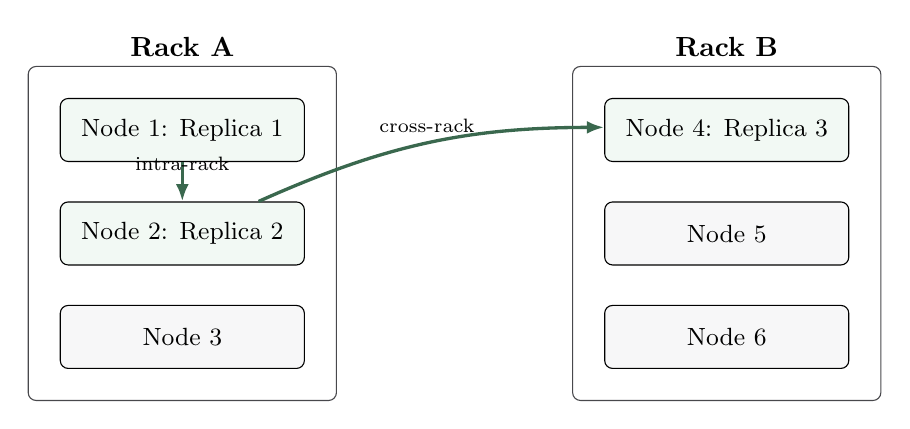
\begin{tikzpicture}[
  rack/.style={draw=RemarkGray, rounded corners=1mm, inner sep=4mm},
  nodebox/.style={draw, rounded corners=1mm, minimum width=3.1cm, minimum height=8mm, align=center, font=\small}
]
\node[nodebox, fill=DataGreen] (a1) {Node 1: Replica 1};
\node[nodebox, fill=DataGreen, below=5mm of a1] (a2) {Node 2: Replica 2};
\node[nodebox, fill=SoftGray, below=5mm of a2] (a3) {Node 3};

\node[nodebox, fill=DataGreen, right=38mm of a1] (b1) {Node 4: Replica 3};
\node[nodebox, fill=SoftGray, below=5mm of b1] (b2) {Node 5};
\node[nodebox, fill=SoftGray, below=5mm of b2] (b3) {Node 6};

\node[rack, fit=(a1)(a2)(a3), label={[font=\bfseries]above:Rack A}] {};
\node[rack, fit=(b1)(b2)(b3), label={[font=\bfseries]above:Rack B}] {};

\draw[dataflow] (a1) -- node[above,font=\scriptsize]{intra-rack} (a2);
\draw[dataflow] (a2) to[bend left=12] node[above,font=\scriptsize]{cross-rack} (b1);
\end{tikzpicture}
\caption{Rack-aware replication with two replicas in one rack and one replica in another rack. The placement balances durability against cross-rack write traffic.}
\label{fig:rack-replication}
\end{figure}

\subsection{Replication Factor Trade-offs}

\begin{definitionbox}{Replication Factor}
The replication factor is the number of copies maintained for each chunk or block.
\end{definitionbox}

\begin{table}[htbp]
\centering
\caption{Replication factor, storage overhead, and simplified durability interpretation.}
\label{tab:replication-factor}
\begin{tabularx}{0.82\textwidth}{C{3.0cm} C{3.0cm} Y}
\toprule
\rowcolor{TableTint}
Replication factor & Storage overhead & Durability \\
\midrule
1 (no replication) & $1\times$ & No redundancy; a failure can lose the only copy \\
2 & $2\times$ & Tolerates one replica failure \\
3 (typical default) & $3\times$ & Tolerates two simultaneous replica failures in the simplified model \\
\bottomrule
\end{tabularx}
\end{table}

Increasing replication improves durability but consumes more storage and adds write traffic. The acknowledgement policy and handling of failed replicas determine when a write is accepted; the configured replication factor need not always be met immediately.

\subsection{Failure Domains}

Replication must consider correlated failures at multiple scales:

\begin{table}[htbp]
\centering
\caption{Failure domains relevant to distributed storage.}
\label{tab:failure-domains}
\begin{tabularx}{0.78\textwidth}{>{\bfseries\raggedright\arraybackslash}p{3.1cm} Y}
\toprule
Failure domain & Scope of impact \\
\midrule
Disk & One local copy of one or more chunks \\
Node & All chunks stored on the failed machine \\
Rack & Multiple machines sharing a switch or power source \\
Datacenter & An entire facility, including power or network loss \\
\bottomrule
\end{tabularx}
\end{table}

Spreading replicas across failure domains is important precisely because failures are not always independent.

\subsection{Worked Example: Replication and Data-Loss Probability}

Consider a simplified one-year model with no repair or re-replication, in which each replica is permanently lost with independent probability \(p=0.02\). For \(r\) replicas, the probability of losing all copies by the end of that year is

\begin{equation}
P(\text{total loss}) = p^r.
\label{eq:replica-loss}
\end{equation}

For \(p=0.02\),

\begin{table}[htbp]
\centering
\caption{Simplified independent-failure illustration for \(p=0.02\).}
\label{tab:replica-prob}
\begin{tabular}{cc}
\toprule
Replication factor \(r\) & \(P(\text{loss}) = p^r\) \\
\midrule
1 & \(0.02\) \\
2 & \(0.0004\) \\
3 & \(0.000008\) \\
\bottomrule
\end{tabular}
\end{table}

\begin{remarkbox}{Simplified independence model}
This no-repair example illustrates the multiplicative effect of independent replicas. It is not an estimate of annual data-loss risk in a self-healing cluster: real durability also depends on repair time, overlapping failures, and shared failure domains.
\end{remarkbox}

\subsection{Re-Replication after Failure}

A failed node does not leave the cluster permanently under-replicated. The recovery process is:

\begin{enumerate}
    \item the Master or NameNode detects the failed node through missed heartbeats;
    \item affected blocks are marked under-replicated;
    \item the system selects surviving replicas;
    \item new copies are scheduled on healthy nodes;
    \item the desired replication factor is restored automatically.
\end{enumerate}

\subsection{Balancing Storage Utilization}

Replica placement and re-replication also consider disk utilization. A balanced cluster avoids concentrating too much data on a small subset of machines, thereby reducing hotspots and premature capacity exhaustion.

\subsubsection*{Review Questions}
\begin{enumerate}
    \item Why is moving computation to data preferable to moving data to computation?
    \item How does rack-aware placement balance durability against write cost?
    \item Under the simplified independent-failure model, why does moving from two to three replicas reduce loss probability so strongly?
    \item What happens after a Chunkserver or DataNode permanently fails?
\end{enumerate}


% ============================================================
\section{Hadoop Distributed File System (HDFS)}
% ============================================================

\subsection{Origins and Relation to GFS}

HDFS was designed as an open-source distributed storage system directly inspired by the 2003 GFS paper. It was built within Apache Hadoop to support large-scale, fault-tolerant batch processing and originally served the MapReduce execution model.

Its central architecture is nearly the same as GFS: one metadata-managing node, many data-storing nodes, large fixed-size blocks, and replication.

\subsection{Architecture}

\begin{figure}[htbp]
\centering
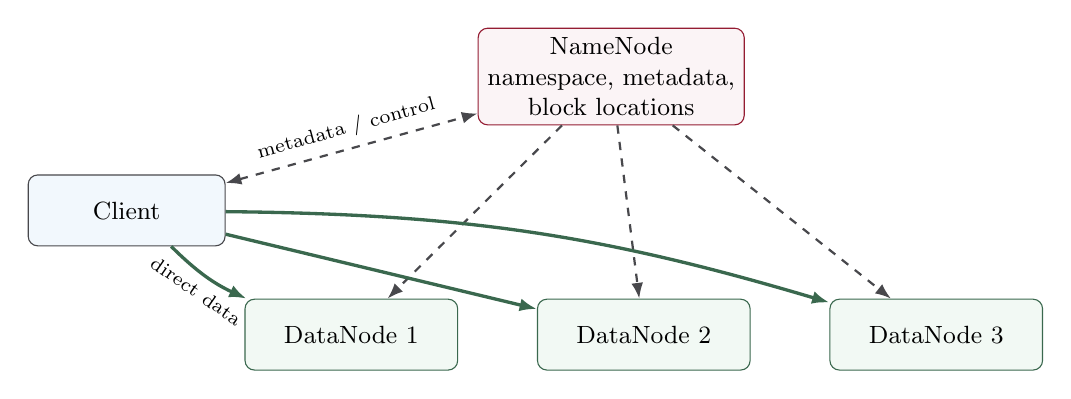
\begin{tikzpicture}[node distance=15mm and 15mm]
\node[clientnode] (client) {Client};
\node[metadata, right=32mm of client, yshift=17mm] (nn) {NameNode\\namespace, metadata,\\block locations};
\node[datanode, below=22mm of nn, xshift=-33mm] (d1) {DataNode 1};
\node[datanode, right=10mm of d1] (d2) {DataNode 2};
\node[datanode, right=10mm of d2] (d3) {DataNode 3};

\draw[controlbi] (client) -- node[above,sloped,font=\scriptsize]{metadata / control} (nn);
\draw[control] (nn) -- (d1);
\draw[control] (nn) -- (d2);
\draw[control] (nn) -- (d3);

\draw[dataflow] (client) to[bend right=10] node[below,sloped,font=\scriptsize]{direct data} (d1);
\draw[dataflow] (client) -- (d2);
\draw[dataflow] (client) to[bend left=8] (d3);
\end{tikzpicture}
\caption{HDFS architecture. The NameNode plays the metadata role of the GFS Master, while DataNodes correspond to GFS Chunkservers.}
\label{fig:hdfs-architecture}
\end{figure}

\subsection{NameNode}

The NameNode maintains the namespace, permissions, file-to-block mappings, block-to-DataNode locations, and coordination decisions for replication, deletion, and rebalancing. The metadata is kept in memory for fast access.

\subsection{DataNodes}

DataNodes store HDFS blocks as files on their local underlying file systems and serve block reads and writes directly to clients. They periodically send heartbeats and block reports to the NameNode.

\subsection{Block Size}

\begin{table}[htbp]
\centering
\caption{GFS chunk size and HDFS block size.}
\label{tab:gfs-hdfs-size}
\begin{tabularx}{0.72\textwidth}{>{\bfseries\raggedright\arraybackslash}p{3.2cm} C{2.7cm} Y}
\toprule
\rowcolor{TableTint}
System & Default size & Typical range \\
\midrule
GFS chunk & 64 MB & Fixed at 64 MB \\
HDFS block & 128 MB & Configurable, commonly 128--256 MB \\
\bottomrule
\end{tabularx}
\end{table}

Both systems use large units for the same reasons: reduced metadata and efficient sequential transfer.

\subsection{FsImage and EditLog}

HDFS persists NameNode metadata using two structures:

\begin{itemize}
    \item \textbf{FsImage:} a complete point-in-time snapshot of the namespace;
    \item \textbf{EditLog:} an append-only log of namespace mutations since the most recent FsImage.
\end{itemize}

This is analogous to GFS's checkpoint plus operation log.

\subsection{NameNode Startup}

On restart, the NameNode loads the most recent FsImage and replays EditLog entries recorded since that snapshot. The resulting in-memory namespace reconstructs the state that existed before the restart. A new checkpoint can then bound future replay time.

\subsection{Secondary NameNode}

\begin{remarkbox}{Secondary NameNode misconception}
The Secondary NameNode is \emph{not} a hot standby and is not the component that automatically takes over when the primary NameNode fails. Its role is to merge FsImage and EditLog periodically into a new checkpoint, thereby offloading checkpointing work.
\end{remarkbox}

\subsection{High Availability}

Production HDFS can use Active/Standby NameNodes. One Active node handles client requests while one or more Standby nodes remain synchronized through a shared, consistent edit log. Automatic failover can promote a Standby when the Active node fails.

\subsection{Heartbeats and Block Reports}

HDFS separates two periodic mechanisms:

\begin{itemize}
    \item \textbf{heartbeats:} frequent liveness messages;
    \item \textbf{block reports:} less frequent full inventories of blocks stored on a DataNode.
\end{itemize}

Together, they allow the NameNode to maintain an accurate view of node health and block distribution.

\subsection{HDFS Read Path}

\begin{enumerate}
    \item The client asks the NameNode for the locations of the blocks that form the target file.
    \item The NameNode returns block identifiers and an ordered list of DataNodes for each block.
    \item The client connects directly to the nearest available DataNode.
    \item The selected DataNode streams block data directly to the client.
\end{enumerate}

\begin{figure}[htbp]
\centering
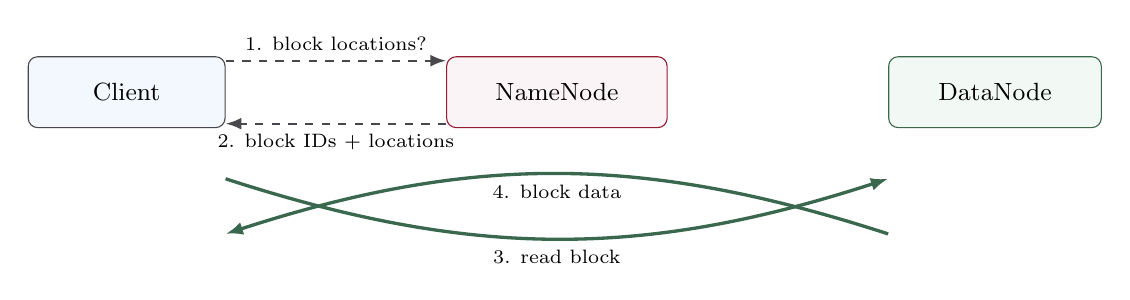
\begin{tikzpicture}[node distance=28mm]
\node[clientnode] (c) {Client};
\node[metadata, right=of c] (n) {NameNode};
\node[datanode, right=of n] (d) {DataNode};

\draw[control] ([yshift=4mm]c.east) -- node[above,font=\scriptsize]{1. block locations?} ([yshift=4mm]n.west);
\draw[control] ([yshift=-4mm]n.west) -- node[below,font=\scriptsize]{2. block IDs + locations} ([yshift=-4mm]c.east);
\draw[dataflow] ([yshift=-11mm]c.east) to[bend right=18] node[below,font=\scriptsize]{3. read block} ([yshift=-11mm]d.west);
\draw[dataflow] ([yshift=-18mm]d.west) to[bend right=18] node[below,font=\scriptsize]{4. block data} ([yshift=-18mm]c.east);
\end{tikzpicture}
\caption{HDFS read path. As in GFS, the metadata lookup is separated from the direct block-data transfer.}
\label{fig:hdfs-read}
\end{figure}

\subsection{HDFS Write Pipeline}

HDFS also uses a node-to-node replication pipeline, but its write protocol is organized differently from GFS: the client streams packets through a DataNode chain and acknowledgements return through that chain, whereas GFS separately uses a lease-holding primary to serialize mutations after the data has been propagated.

\begin{enumerate}
    \item The client asks the NameNode to create a file; the NameNode checks permissions and allocates a block.
    \item The NameNode returns DataNodes that form the replication pipeline.
    \item The client streams data to the first DataNode.
    \item Each DataNode forwards the data to the next DataNode.
    \item Acknowledgements return in the reverse direction after the pipeline has processed the packets. An ordinary acknowledgement does not imply a disk-device sync; \texttt{hsync()} provides that stronger synchronization request.
\end{enumerate}

\begin{figure}[htbp]
\centering
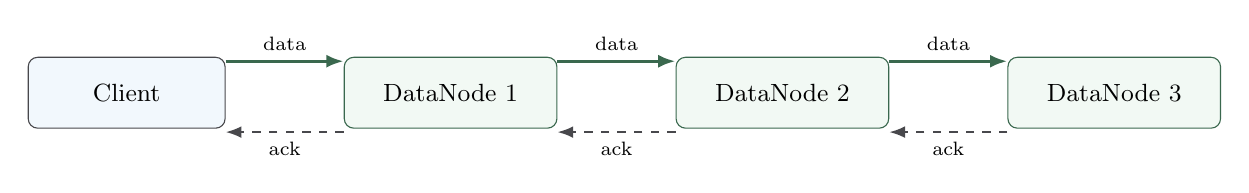
\begin{tikzpicture}[node distance=15mm]
\node[clientnode] (c) {Client};
\node[datanode, right=of c] (d1) {DataNode 1};
\node[datanode, right=of d1] (d2) {DataNode 2};
\node[datanode, right=of d2] (d3) {DataNode 3};

\draw[dataflow] ([yshift=4mm]c.east) -- node[above,font=\scriptsize]{data} ([yshift=4mm]d1.west);
\draw[dataflow] ([yshift=4mm]d1.east) -- node[above,font=\scriptsize]{data} ([yshift=4mm]d2.west);
\draw[dataflow] ([yshift=4mm]d2.east) -- node[above,font=\scriptsize]{data} ([yshift=4mm]d3.west);

\draw[control] ([yshift=-5mm]d3.west) -- node[below,font=\scriptsize]{ack} ([yshift=-5mm]d2.east);
\draw[control] ([yshift=-5mm]d2.west) -- node[below,font=\scriptsize]{ack} ([yshift=-5mm]d1.east);
\draw[control] ([yshift=-5mm]d1.west) -- node[below,font=\scriptsize]{ack} ([yshift=-5mm]c.east);
\end{tikzpicture}
\caption{HDFS write pipeline. Data flows through a chain of DataNodes and acknowledgements return in the reverse direction.}
\label{fig:hdfs-write}
\end{figure}

\subsection{Replica Placement Policy}

For replication factor three, HDFS uses the following rack-aware placement pattern:

\begin{enumerate}
    \item first replica on the local or a nearby DataNode;
    \item second replica on a different rack;
    \item third replica on a different node in the same rack as the second.
\end{enumerate}

This preserves cross-rack durability while limiting the number of cross-rack transfers.

Rack awareness must be configured explicitly. Without a mapping from DataNodes to racks, HDFS may treat the cluster as a single rack and lose the intended protection against rack-level failures.

\subsection{Federation}

HDFS Federation addresses NameNode metadata scalability by introducing multiple independent NameNodes. Each manages a distinct portion of the namespace, while DataNodes register with and store blocks for all NameNodes in the federation.

Each NameNode still has its own in-memory limit, but aggregate namespace capacity scales with the number of NameNodes.

\subsection{GFS and HDFS: Terminology and Architecture}

\begin{table}[htbp]
\centering
\caption{Terminology mapping between GFS and HDFS.}
\label{tab:terminology-mapping}
\begin{tabularx}{0.80\textwidth}{>{\bfseries}Y Y Y}
\toprule
\rowcolor{TableTint}
Concept & GFS term & HDFS term \\
\midrule
Metadata node & Master & NameNode \\
Data-storing node & Chunkserver & DataNode \\
Storage unit & Chunk & Block \\
Default unit size & 64 MB & 128 MB \\
Recovery / checkpoint support & Shadow masters (read-only replicas) & Secondary NameNode (checkpoint helper) \\
\bottomrule
\end{tabularx}
\end{table}

\begin{remarkbox}{No exact one-to-one equivalent}
GFS shadow masters and the HDFS Secondary NameNode solve different supporting problems. Shadow masters maintain read-only replicas of Master state, whereas the Secondary NameNode periodically merges the FsImage and EditLog to create checkpoints; neither should be interpreted as a simple hot-standby equivalent of the other.
\end{remarkbox}

\begin{table}[htbp]
\centering
\caption{Architectural comparison between GFS and HDFS.}
\label{tab:gfs-hdfs-comparison}
\begin{tabularx}{\textwidth}{>{\bfseries\raggedright\arraybackslash}p{3.1cm} Y Y}
\toprule
\rowcolor{TableTint}
Aspect & GFS & HDFS \\
\midrule
Metadata coordinator & Master & NameNode \\
Data node & Chunkserver & DataNode \\
Storage unit & Chunk & Block \\
Default unit size & 64 MB & 128 MB \\
Write coordination & Pipelined data propagation; primary/lease serializes mutations & Client-to-DataNode pipeline with reverse acknowledgements \\
Metadata persistence & Checkpoint + operation log & FsImage + EditLog \\
Metadata scaling & Single-Master limitations & Federation adds multiple NameNodes \\
Availability & Shadow masters plus recovery/promotion mechanisms & Explicit Active/Standby HA configuration \\
\bottomrule
\end{tabularx}
\end{table}

\subsection{Why Blocks Suit Batch Processing}

Blocks are independently processable units. Their physical locations can be exposed to a scheduler, which enables one task to be placed near the block it processes. This storage abstraction therefore leads directly to MapReduce-style parallelism.

\subsection{Append-Only, No Random Writes}

HDFS follows the same write-once-read-many philosophy introduced earlier. Append operations are supported, but arbitrary in-place modification of existing file contents is not part of the classic model. This restriction simplifies consistency and replication.

\subsubsection*{Review Questions}
\begin{enumerate}
    \item Map NameNode, DataNode, and block to their GFS counterparts.
    \item What is the actual role of the Secondary NameNode?
    \item How do the HDFS and GFS write protocols differ in control and ordering, even though both use pipelined data propagation?
    \item How does Federation address the NameNode metadata bottleneck?
    \item Why does block-based storage naturally support parallel batch computation?
\end{enumerate}


% ============================================================
\section{Failure Handling and Fault Tolerance}
% ============================================================

\subsection{Failure Is the Default Assumption}

With thousands of disks and machines, failures are a continuous background process. Replication, heartbeats, leases, logs, checkpoints, and checksums exist so that the system can degrade and recover gracefully rather than depend on the absence of failure.

\subsection{Types of Failures}

Failures can be divided into three broad categories:

\begin{itemize}
    \item \textbf{Transient failures:} temporary network interruptions or brief pauses;
    \item \textbf{Permanent failures:} disk death, hardware failure, or node decommissioning;
    \item \textbf{Correlated failures:} failures affecting multiple machines simultaneously, such as rack power or switch loss.
\end{itemize}

\subsection{Detecting Failure: Heartbeats and Timeouts}

Each data node sends periodic heartbeats to the metadata node. If no heartbeat arrives before a timeout, the node is presumed dead.

\begin{table}[htbp]
\centering
\caption{Heartbeat timeout trade-off.}
\label{tab:timeout-tradeoff}
\begin{tabularx}{0.92\textwidth}{>{\bfseries\raggedright\arraybackslash}p{2.2cm} Y Y}
\toprule
\rowcolor{TableTint}
Timeout & Detection behaviour & Main risk \\
\midrule
Short & Fast failure detection & False positives for slow but healthy nodes; unnecessary re-replication \\
Long & Fewer false positives & Slower detection of real failures; longer period of reduced redundancy \\
\bottomrule
\end{tabularx}
\end{table}

There is no universally correct timeout; it must be chosen for the cluster's workload and network conditions.

\subsection{Recovery from Chunkserver / DataNode Failure}

The recovery chain is:

\[
\begin{aligned}
\text{missed heartbeat}
&\Longrightarrow \text{node presumed dead}
\Longrightarrow \text{blocks marked under-replicated} \\
&\Longrightarrow \text{new replicas scheduled}
\Longrightarrow \text{replication factor restored}.
\end{aligned}
\]

\begin{figure}[htbp]
\centering
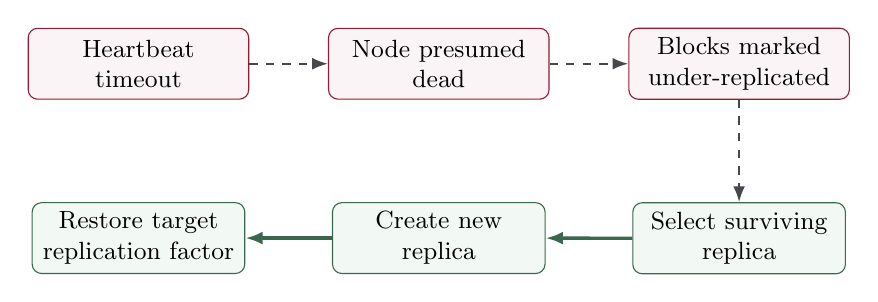
\begin{tikzpicture}[node distance=10mm]
\node[metadata] (h) {Heartbeat\\timeout};
\node[metadata, right=of h] (d) {Node presumed\\dead};
\node[metadata, right=of d] (u) {Blocks marked\\under-replicated};
\node[datanode, below=13mm of u] (r) {Select surviving\\replica};
\node[datanode, below=13mm of d] (n) {Create new\\replica};
\node[datanode, below=13mm of h] (f) {Restore target\\replication factor};

\draw[control] (h) -- (d);
\draw[control] (d) -- (u);
\draw[control] (u) -- (r);
\draw[dataflow] (r) -- (n);
\draw[dataflow] (n) -- (f);
\end{tikzpicture}
\caption{Simplified self-healing chain after a data-storage node failure.}
\label{fig:rereplication}
\end{figure}

\subsection{Recovery from Master / NameNode Failure}

Without high availability, the cluster cannot accept new operations until the metadata node is restarted and its state reconstructed from a checkpoint plus log. With HA configured, a synchronized Standby can be promoted to Active, greatly reducing interruption.

\subsection{Checksums and Silent Corruption}

Crashes are not the only failure mode. A disk may return corrupted data without reporting a hardware error. Both GFS and HDFS therefore store checksums alongside chunks or blocks.

A read verifies the checksum. If a mismatch is detected, another valid replica is used and the corrupted replica can be replaced.

\[
\begin{aligned}
\text{read block}
&\Longrightarrow \text{verify checksum}
\Longrightarrow \text{detect mismatch} \\
&\Longrightarrow \text{read valid replica}
\Longrightarrow \text{regenerate replica}.
\end{aligned}
\]

\begin{keyconcept}
Heartbeats detect missing nodes; block reports describe data placement; checksums detect silent corruption; re-replication restores the desired redundancy. Together these mechanisms produce the self-healing behaviour of the storage system.
\end{keyconcept}

\subsection{Real-World Failure Rates at Scale}

Disk failure rates are often summarized using an Annualized Failure Rate (AFR). The supplied material uses a representative range of roughly \(1\%\) to \(5\%\) AFR, depending on disk age, model, and operating conditions.

The worked example uses \(10{,}000\) disks and a \(2\%\) annual failure rate.

\subsection{Modeling Disk Failures in One Week}

Consider

\[
N = 10{,}000
\]

disks with annual failure rate

\[
\mathrm{AFR}=2\%=0.02.
\]

Let \(p\) denote the probability that one disk fails during one week. Under the simplifying assumption that failures are uniformly distributed throughout the year,

\begin{equation}
p \approx \frac{0.02}{52}
  \approx 0.0003846.
\label{eq:weekly-failure-prob}
\end{equation}

For each disk, define the indicator variable

\begin{equation}
X_i =
\begin{cases}
1, & \text{if disk } i \text{ fails during the week},\\
0, & \text{otherwise}.
\end{cases}
\label{eq:indicator}
\end{equation}

Then

\[
X_i \sim \operatorname{Bernoulli}(p).
\]

The total number of failures in the week is

\begin{equation}
X = \sum_{i=1}^{N} X_i.
\label{eq:total-failures}
\end{equation}

Under the stated assumption that the disk failures are independent and identically distributed,

\begin{equation}
X \sim \operatorname{Binomial}(N,p),
\qquad
N=10{,}000,
\quad
p\approx 0.0003846.
\label{eq:binomial-model}
\end{equation}

\subsection{Probability of Exactly \texorpdfstring{$k$}{k} Failures}

For a binomial random variable,

\begin{equation}
\Pr(X=k)
=
\binom{N}{k}
p^k
(1-p)^{N-k}.
\label{eq:binomial-pmf}
\end{equation}

For exactly four failures in one week,

\[
\Pr(X=4)
=
\binom{10{,}000}{4}
(0.0003846)^4
(1-0.0003846)^{9996}
\approx 19.5\%.
\]

Thus, under this simplified model, exactly four failures in a week is not an unusual outcome.

\subsection{Expected Number of Failures}

For a binomial random variable,

\begin{equation}
\mathbb{E}[X]=Np.
\label{eq:binomial-expectation}
\end{equation}

Therefore,

\[
\mathbb{E}[X]
=
10{,}000\cdot\frac{0.02}{52}
\approx 3.85.
\]

An important interpretation is that

\[
\mathbb{E}[X]\approx 3.85
\qquad\not\Rightarrow\qquad
X=3.85.
\]

The random variable \(X\) takes integer values,

\[
X\in\{0,1,2,3,\ldots,N\},
\]

whereas \(3.85\) is the long-run average.

\subsection{Variance and Standard Deviation}

For a binomial random variable,

\begin{equation}
\operatorname{Var}(X)=Np(1-p).
\label{eq:binomial-variance}
\end{equation}

With these values,

\[
\operatorname{Var}(X)
=
10{,}000(0.0003846)(1-0.0003846)
\approx 3.84.
\]

Hence,

\[
\sigma_X
=
\sqrt{\operatorname{Var}(X)}
\approx 1.96.
\]

The weekly number of failures therefore fluctuates naturally around its expectation.

\subsection{From AFR to Failures per Week}

The complete chain is

\[
\mathrm{AFR}=0.02,
\qquad
p_{\text{week}}\approx\frac{0.02}{52}\approx0.0003846,
\]

\[
X\sim\operatorname{Binomial}(10{,}000,0.0003846),
\]

and

\[
\mathbb{E}[X]=Np\approx3.85.
\]

This is the central scaling effect: a small annual probability for one disk becomes a regular stream of failures when the number of disks is very large.

\subsection{Probability of at Least One Failure}

The probability of at least one failure is most conveniently computed using the complement:

\begin{equation}
\Pr(X\geq 1)
=
1-\Pr(X=0).
\label{eq:at-least-one}
\end{equation}

For a binomial random variable,

\[
\Pr(X=0)=(1-p)^N,
\]

so

\begin{equation}
\Pr(X\geq 1)
=
1-(1-p)^N.
\label{eq:at-least-one-binomial}
\end{equation}

Substituting these values,

\[
\Pr(X\geq 1)
=
1-(1-0.0003846)^{10{,}000}
\approx 97.9\%.
\]

Thus, under the stated simplifying assumptions, a cluster of \(10{,}000\) disks experiences at least one disk failure in roughly \(98\%\) of weeks.

\begin{remarkbox}{Model assumptions}
The calculation deliberately uses a simplified iid model and the approximation \(p\approx \mathrm{AFR}/52\). Its purpose is to quantify the scaling effect, not to provide a complete empirical model of correlated or age-dependent disk failures.
\end{remarkbox}

\subsection{Example: Chunkserver Dies Mid-Read}

\begin{examplebox}{Chunkserver failure during an active read}
Suppose a client is reading a chunk from Chunkserver A and A crashes during the transfer.

\textbf{Client-visible sequence:}
\begin{enumerate}
    \item the current transfer fails or times out;
    \item the client re-queries the Master for alternative replica locations;
    \item the client retries the read against another Chunkserver, such as B or C;
    \item the application-level read succeeds using the surviving replica.
\end{enumerate}

\textbf{Background recovery sequence:}
\begin{enumerate}
    \item the Master notices A's missed heartbeats;
    \item chunks formerly stored on A are marked under-replicated;
    \item re-replication is scheduled from surviving copies to healthy nodes.
\end{enumerate}
\end{examplebox}

\subsubsection*{Review Questions}
\begin{enumerate}
    \item Why must heartbeat timeouts balance detection speed against false positives?
    \item What happens after a DataNode permanently fails?
    \item Why are checksums necessary even when data is replicated?
    \item Why does a cluster of thousands of disks experience failures on a weekly rather than yearly timescale?
    \item In the mid-read failure example, which steps are visible to the client and which happen in the background?
\end{enumerate}


% ============================================================
\section{From Storage to Computation}
% ============================================================

\subsection{GFS and HDFS Side by Side}

\begin{figure}[htbp]
\centering
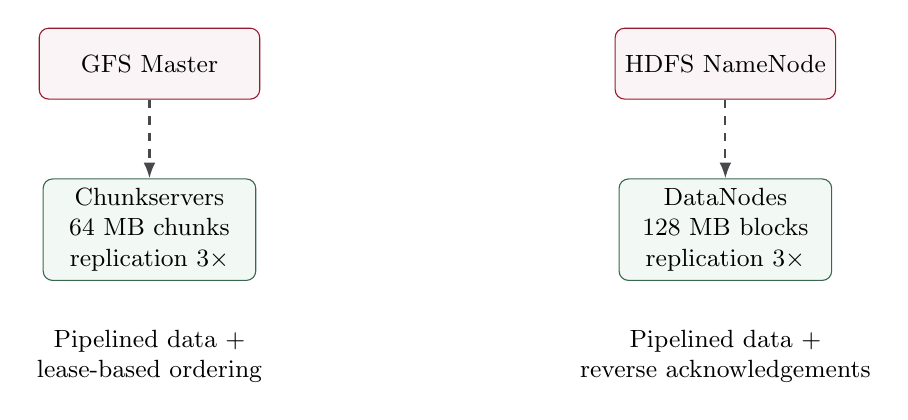
\begin{tikzpicture}[node distance=10mm and 26mm]
\node[metadata] (gm) {GFS Master};
\node[datanode, below=of gm] (gcs) {Chunkservers\\64 MB chunks\\replication $3\times$};

\node[metadata, right=45mm of gm] (hn) {HDFS NameNode};
\node[datanode, below=of hn] (hdn) {DataNodes\\128 MB blocks\\replication $3\times$};

\draw[control] (gm) -- (gcs);
\draw[control] (hn) -- (hdn);

\node[below=5mm of gcs, font=\small, align=center] {Pipelined data +\\lease-based ordering};
\node[below=5mm of hdn, font=\small, align=center] {Pipelined data +\\reverse acknowledgements};
\end{tikzpicture}
\caption{High-level GFS/HDFS architectural recap. Both systems separate metadata coordination from replicated data storage and use pipelined replication, while their write-control mechanisms differ.}
\label{fig:gfs-hdfs-recap}
\end{figure}

The two systems share the same core architectural idea even though terminology and some mechanics differ.

\subsection{Storage Enables Compute}

The storage design is significant because it directly enables distributed computation:

\[
\text{fixed-size blocks}
\Longrightarrow
\text{parallel units of computation},
\]

\[
\text{known block locations}
\Longrightarrow
\text{data-local scheduling},
\]

\[
\text{replicated, fault-tolerant storage}
\Longrightarrow
\text{reliable substrate for distributed computation}.
\]

A computation framework does not need to invent its own storage layer. It can schedule work over data already distributed and protected by GFS or HDFS.

\subsection{MapReduce on Top of Distributed Storage}

MapReduce builds a computation layer directly on top of this storage foundation. A MapReduce job reads data stored as blocks or chunks, and Map tasks can be placed on or near the machines that hold those inputs. Outputs are written back to the distributed file system and inherit its replication and fault-tolerance mechanisms.

The following chapter develops the Map, Shuffle, Sort, and Reduce execution model in detail; the essential connection is that computation inherits the storage layer's block structure, locality information, and fault-tolerant substrate.

\subsection{Limits of the GFS/HDFS Model}

This architecture has several important limitations:

\begin{itemize}
    \item optimization for large files and sequential access makes the model a poor fit for very large numbers of small files or random-access workloads;
    \item a centralized metadata architecture imposes namespace scalability limits, even when HA and Federation mitigate different aspects of the problem;
    \item write-once-read-many semantics are restrictive for workloads requiring frequent in-place updates.
\end{itemize}

Later topics such as Spark, streaming, and lakehouse architectures address different parts of this design space.

\subsection{Three Pillars of Scale-Out Storage}

The architecture can be distilled into three structural principles:

\begin{enumerate}
    \item \textbf{Horizontal scaling over commodity hardware:} many inexpensive, individually unreliable machines rather than a few expensive machines.
    \item \textbf{Block-based storage with replication:} fixed-size units simplify placement, parallelism, durability, and recovery.
    \item \textbf{Separated metadata management and data transfer:} a coordinating node tracks locations and namespace state, while bulk data flows directly between clients and data-storing nodes.
\end{enumerate}

% ============================================================
\section{Key Terms}
% ============================================================

\begin{table}[htbp]
\centering
\caption{Key terminology for scale-out distributed storage.}
\label{tab:storage-key-terms}
\begin{tabularx}{\textwidth}{>{\bfseries\raggedright\arraybackslash}p{4.0cm} Y}
\toprule
Term & Meaning \\
\midrule
Scale up & Increase the capacity of one machine. \\
Scale out & Increase capacity by adding machines to a cluster. \\
Distributed File System & Logical file system backed by storage distributed across many machines. \\
Chunk / Block & Fixed-size unit of distributed file storage; 64 MB in GFS and 128 MB by default in the HDFS material. \\
Master / NameNode & Metadata-managing coordinator. \\
Chunkserver / DataNode & Node storing and serving actual data. \\
Replication factor & Number of copies maintained for each chunk or block. \\
Heartbeat & Periodic liveness signal from a data node to the coordinator. \\
Block report & HDFS report containing the blocks held by a DataNode. \\
Data locality & Scheduling computation near the data it consumes. \\
Rack awareness & Placement strategy that accounts for physical failure and bandwidth domains. \\
Lease & Time-bounded designation of a GFS replica as primary for ordering mutations. \\
FsImage & Point-in-time snapshot of the HDFS namespace. \\
EditLog & Append-only log of HDFS namespace mutations. \\
Re-replication & Automatic reconstruction of lost or corrupted replicas. \\
Checksum & Integrity value used to detect silent data corruption. \\
\bottomrule
\end{tabularx}
\end{table}

% ============================================================
\section{Chapter Summary}
% ============================================================

\begin{longtable}{>{\bfseries\raggedright\arraybackslash}p{\dimexpr0.235\textwidth-2\tabcolsep\relax} >{\raggedright\arraybackslash}p{\dimexpr0.35\textwidth-2\tabcolsep\relax} >{\raggedright\arraybackslash}p{\dimexpr0.415\textwidth-2\tabcolsep\relax}}
\caption{Compact summary of the central relationships in scale-out distributed storage.}
\label{tab:storage-core-relationships}\\
\toprule
Concept & Main role & Important relationship / trade-off \\
\midrule
\endfirsthead
\toprule
Concept & Main role & Important relationship / trade-off \\
\midrule
\endhead
Scale Up & Grow one machine & Simple software model, but high-end cost grows steeply and physical limits remain. \\
Scale Out & Grow a cluster & Capacity grows by adding nodes, but distributed coordination becomes necessary. \\
Commodity hardware & Cheap cluster components & Reliability moves from individual hardware into distributed software mechanisms. \\
Large blocks / chunks & Storage unit & Reduce metadata and favour sequential I/O, but are inefficient for small-file workloads. \\
Metadata coordinator & Track namespace and locations & Central coordination is simple and fast but may become a bottleneck and availability concern. \\
Direct data transfer & Keep bulk bytes off metadata node & Prevents the coordinator from becoming a throughput bottleneck. \\
Replication & Provide redundancy & Improves durability at the cost of storage capacity and write traffic. \\
Rack awareness & Spread replicas across failure domains & Balances correlated-failure protection against cross-rack bandwidth cost. \\
Data locality & Place computation near data & Reduces network transfer of large input datasets. \\
GFS Master & Manage GFS metadata & Uses in-memory metadata, operation log, checkpoints, leases, and Chunkserver reports. \\
GFS Chunkserver & Store GFS chunks & Serves data directly and reports chunk state to the Master. \\
HDFS NameNode & Manage HDFS metadata & Uses in-memory state plus FsImage/EditLog; HA and Federation address availability and scaling separately. \\
HDFS DataNode & Store HDFS blocks & Serves blocks directly and sends heartbeats plus block reports. \\
GFS write path & Order mutations & Client pushes data to replicas; a leased primary serializes mutation order. \\
HDFS write path & Replicate data & Data streams through a DataNode pipeline and acknowledgements return backwards. \\
Heartbeat & Detect suspected failure & Short timeouts detect quickly but risk false positives; long timeouts delay recovery. \\
Checksum & Detect silent corruption & Complements replication by detecting bad copies that still appear reachable. \\
Re-replication & Restore redundancy & Converts surviving replicas into replacement copies after failure or corruption. \\
FsImage + EditLog & Persist HDFS namespace & Snapshot plus mutation log reconstructs the NameNode's in-memory state. \\
Secondary NameNode & Checkpoint helper & Merges FsImage and EditLog; it is not the HA standby. \\
Federation & Scale HDFS namespace & Multiple independent NameNodes increase aggregate namespace capacity. \\
High Availability & Reduce metadata-node downtime & Active/Standby NameNodes allow failover with synchronized edits. \\
Block-based storage & Foundation for batch processing & Independent blocks support parallel tasks and data-local scheduling. \\
\bottomrule
\end{longtable}

% ============================================================
\section{Quick Review}
% ============================================================

\begin{enumerate}
    \item Big data infrastructure begins from the assumption that no single machine is infinitely large, fast, or reliable.
    \item Vertical scaling enlarges one machine; horizontal scaling adds machines.
    \item Scale up is simple but eventually reaches both economic and physical ceilings.
    \item Scale out relies on software-level coordination and fault tolerance over commodity hardware.
    \item At cluster scale, component failure is normal rather than exceptional.
    \item Big data DFSs optimize aggregate throughput rather than minimum single-request latency.
    \item Their intended workload contains very large files, sequential access, and write-once-read-many behaviour.
    \item Fixed-size blocks or chunks simplify metadata, placement, replication, load balancing, and recovery.
    \item Metadata is separated from bulk data so that the coordinator performs lookups rather than carrying file contents.
    \item GFS uses a Master and Chunkservers; HDFS uses a NameNode and DataNodes.
    \item GFS uses 64 MB chunks; HDFS uses a 128 MB default block size in this material.
    \item GFS keeps Master metadata in memory for speed and persists namespace mutations through an operation log and checkpoints.
    \item GFS clients obtain chunk metadata from the Master but transfer data directly with Chunkservers.
    \item GFS writes decouple data transfer from mutation ordering; a leased primary orders writes for secondary replicas.
    \item HDFS persists namespace state through FsImage and EditLog.
    \item The Secondary NameNode is a checkpointing helper, not a hot standby.
    \item HDFS HA uses Active and Standby NameNodes; Federation uses multiple NameNodes to scale namespace capacity.
    \item Both GFS and HDFS pipeline replica data; GFS additionally uses a lease-holding primary to serialize mutations, while HDFS uses a DataNode pipeline with reverse acknowledgements.
    \item Replication improves durability but consumes storage and increases write traffic.
    \item Rack-aware placement spreads replicas across failure domains while limiting cross-rack communication.
    \item Data locality reduces network traffic by scheduling computation near the blocks it needs.
    \item Heartbeats detect missing nodes; block reports describe stored data; checksums detect silent corruption.
    \item Re-replication restores the intended replication factor after failure or corruption.
    \item A short heartbeat timeout improves detection speed but increases false positives; a long timeout has the opposite trade-off.
    \item Under the simplified model, \(10{,}000\) disks with \(2\%\) AFR yield an expected \(3.85\) failures per week and roughly \(97.9\%\) probability of at least one weekly failure.
    \item The block abstraction naturally supports parallel batch computation and data-local Map scheduling.
    \item MapReduce is built on top of the storage mechanisms introduced here rather than replacing them.
\end{enumerate}

% ============================================================
\section{Further Reading}
% ============================================================

Further reading includes:

\begin{itemize}
    \item Ghemawat, S., Gobioff, H., \& Leung, S.-T. (2003). \href{https://research.google/pubs/the-google-file-system/}{\emph{The Google File System}}. SOSP, especially Sections 2.5--2.7 and 3.1--3.3.
    \item Apache Hadoop. \href{https://hadoop.apache.org/docs/stable/hadoop-project-dist/hadoop-hdfs/HdfsDesign.html}{\emph{HDFS Architecture}}.
    \item Apache Hadoop. \href{https://hadoop.apache.org/docs/stable/api/org/apache/hadoop/fs/FSDataOutputStream.html}{\emph{FSDataOutputStream API}}, including \texttt{hflush()} and \texttt{hsync()}.
\end{itemize}




\chapter{The MapReduce Execution Model}
\label{chap:mapreduce}

Distributed storage solves the problem of retaining datasets that exceed the capacity of a single machine, but stored data still needs to be processed. A computation framework must partition work, place tasks near data, move intermediate results, coordinate aggregation, and recover from worker failures without forcing every programmer to implement those mechanisms manually.

MapReduce addresses this problem with a deliberately small programming interface. Users provide Map and Reduce functions, while the runtime transforms those functions into many parallel tasks, schedules them across a cluster, routes intermediate records by key, and reconstructs work after failures. The result is a batch-processing model in which simple deterministic computations can be executed across thousands of unreliable machines.

\begin{keyconcept}
MapReduce separates application logic from distributed execution. The programmer specifies how records are transformed and aggregated; the runtime supplies task scheduling, communication, grouping, fault recovery, and data-local placement.
\end{keyconcept}

\section{The MapReduce Abstraction}
% ============================================================

\subsection{The Problem Being Solved}

Before a reusable framework, every large-scale batch-processing program had to solve the same distributed problems:

\begin{itemize}
    \item split work across machines;
    \item detect and recover from worker failure;
    \item move intermediate results between machines;
    \item combine partial results;
    \item coordinate completion.
\end{itemize}

MapReduce moves these concerns into the framework so that application programmers can concentrate on task-specific logic.

\subsection{Functional Programming Roots}

The model borrows two familiar higher-order operations:

\[
\operatorname{map}(f,L):
\quad
\text{apply }f\text{ independently to each element of }L,
\]

and

\[
\operatorname{reduce}(g,L):
\quad
\text{combine elements of }L\text{ into an aggregate result using }g.
\]

The absence of dependencies among independent map applications is especially important: independent records can be processed in parallel and in arbitrary order.

\subsection{The Programming Model}

From the user's perspective, a MapReduce job is primarily defined by two functions:

\begin{equation}
\operatorname{map}(k,v)
\longrightarrow
[(k'_1,v'_1),\ldots,(k'_m,v'_m)]
\label{eq:map-signature}
\end{equation}

and

\begin{equation}
\operatorname{reduce}\!\left(k', [v'_1,\ldots,v'_n]\right)
\longrightarrow
[\text{output values}].
\label{eq:reduce-signature}
\end{equation}

The programmer does not explicitly write network protocols, worker scheduling, retry logic, or task placement.

\begin{definitionbox}{Map Function}
The Map function processes one input \((key,value)\) pair independently and emits zero, one, or many intermediate \((key,value)\) pairs.
\end{definitionbox}

\begin{definitionbox}{Reduce Function}
The Reduce function receives one intermediate key together with the complete collection of intermediate values associated with that key and emits the final output value or values for that key.
\end{definitionbox}

\subsection{Map Semantics}

Each Map invocation has no visibility into unrelated input records and cannot rely on mutable state produced by other Map calls. That independence allows the runtime to schedule millions of Map invocations across workers in any order.

\subsection{Reduce Semantics}

All values belonging to the same intermediate key are grouped before the Reduce call. Different keys are independent and can therefore be processed by different Reduce tasks in parallel.

% ============================================================
\subsection{Worked Example: Word Count}
% ============================================================

The canonical example counts every word across a large collection of documents.

Suppose the input consists of document identifier and document text pairs. The Map logic is

\[
\operatorname{map}(\text{document\_id},\text{document\_text})
\]

with the operational rule

\[
\text{for each word }w:
\qquad
\operatorname{emit}(w,1).
\]

No global counting occurs during Map. The Map function merely reports one observation per encountered word.

Reduce receives one word and the complete list of counts produced for that word:

\[
\operatorname{reduce}(w,[1,1,\ldots,1])
\]

and computes

\[
\text{total}=\sum_i 1,
\qquad
\operatorname{emit}(w,\text{total}).
\]

\begin{examplebox}{Word Count}
For documents containing the word \texttt{the} several times, each Map task emits \((\texttt{the},1)\) independently. The framework later guarantees that every value associated with \texttt{the} reaches the same Reduce call, where the values are summed.
\end{examplebox}

\subsection{Second Example: Inverted Index}

The same abstraction can build an inverted index:

\[
\operatorname{map}(\text{document\_id},\text{document\_text})
\]

emits

\[
(w,\text{document\_id})
\]

for each word \(w\). Reduce receives all document identifiers associated with a word and emits a unique, sorted list.

The execution model does not change; only the intermediate values and aggregation logic differ.

\subsection{What the Abstraction Hides}

The programmer does not specify:

\begin{itemize}
    \item which worker runs a particular Map or Reduce call;
    \item how intermediate data moves physically;
    \item how to recover from worker crashes;
    \item how values are grouped by key.
\end{itemize}

These responsibilities belong to the MapReduce runtime.

% ============================================================
\subsection{Determinism and Side Effects}
% ============================================================

Determinism is a central assumption for fault tolerance. Given the same input, a re-executed task must reproduce the same output.

\begin{definitionbox}{Deterministic, Side-Effect-Free Task}
A Map or Reduce computation is suitable for transparent re-execution when its result is determined by its input and it does not rely on or mutate external state in a way that changes the observable result of a retry.
\end{definitionbox}

If a worker fails, the runtime can rerun the task elsewhere. This retry strategy is safe because the repeated computation is expected to produce the same logical output.

\begin{keyconcept}
MapReduce fault tolerance relies on the ability to re-execute work. Deterministic and side-effect-free user functions make ``just run the task again'' a valid recovery strategy.
\end{keyconcept}

\subsubsection*{Review Questions}
\begin{enumerate}
    \item What are the signatures and roles of the Map and Reduce functions?
    \item In word count, what does Map emit, and why does it not perform the global count?
    \item Why must Map and Reduce be deterministic and side-effect-free?
    \item Which distributed-systems concerns are hidden from the programmer?
\end{enumerate}


% ============================================================
\section{Execution Architecture}
% ============================================================

\subsection{From Program to Cluster Job}

Turning the user's functions into a distributed job involves a pipeline:

\begin{enumerate}
    \item split input into independent pieces;
    \item create and schedule Map tasks;
    \item partition and shuffle intermediate output;
    \item group and sort intermediate keys;
    \item run Reduce tasks;
    \item write final output.
\end{enumerate}

\subsection{The Master / JobTracker}

A central coordinator, called the Master in Google's original implementation or the JobTracker in Hadoop MapReduce v1, manages the computation:

\begin{itemize}
    \item creates Map and Reduce tasks;
    \item assigns them to workers;
    \item tracks progress;
    \item detects worker failure;
    \item reschedules work after failure.
\end{itemize}

Conceptually, this resembles the coordination role of the GFS Master or HDFS NameNode, but it manages \emph{computation} rather than the storage namespace.

\subsection{Input Splits Become Map Tasks}

MapReduce creates one Map task per logical input split. Splits often follow GFS/HDFS block boundaries, but they are not identical to physical blocks: the input format, compression, and record boundaries affect splitting.

\[
\text{distributed storage block}
\Longrightarrow
\text{natural unit of Map parallelism}.
\]

This coupling is intentional: MapReduce and GFS were designed together.

\subsection{Data Locality in Scheduling}

The coordinator attempts to schedule each Map task on the worker storing its input. If no perfectly local worker is available, it prefers a worker in the same rack before falling back to a more distant machine.

\begin{keyconcept}
The principle ``move computation to data'' becomes a concrete scheduling rule in MapReduce: place Map tasks near the blocks they process.
\end{keyconcept}

\subsection{Number of Map Tasks versus Machines}

The number of Map tasks may be far larger than the number of workers. For example, thousands of blocks can produce thousands of Map tasks on a cluster containing only hundreds of machines. Tasks therefore run in successive waves.

This over-decomposition improves load balancing and later helps straggler mitigation: work is divided into units small enough to redistribute.

\subsection{Intermediate Output Stays Local}

Map output is temporary and is written to the local disk of the worker that executed the Map task rather than directly to the distributed file system.

The reason is economic: intermediate data is required only until the Reduce stage. Replicating it through HDFS/GFS would introduce unnecessary storage and network overhead.

\subsection{Partitioning Intermediate Keys}

All intermediate pairs sharing the same key must reach the same Reduce task. A partition function maps each intermediate key to a reducer.

The default strategy is hash partitioning:

\begin{equation}
\operatorname{partition}(k)
=
\operatorname{hash}(k)
\bmod R,
\label{eq:partition}
\end{equation}

where \(R\) is the number of Reduce tasks.

Because the function is deterministic, identical keys emitted by different Map tasks map to the same reducer.

\begin{definitionbox}{Partition Function}
A partition function assigns every intermediate key to exactly one Reduce-task partition. It therefore determines where the values associated with a key are routed during shuffle.
\end{definitionbox}

\subsection{Choosing the Number of Reduce Tasks}

Unlike the number of Map tasks, which is determined by input splits, the number of Reduce tasks is typically user-controlled.

\begin{table}[htbp]
\centering
\caption{Trade-off in choosing the number of Reduce tasks.}
\label{tab:reducers-tradeoff}
\begin{tabularx}{\textwidth}{>{\bfseries\raggedright\arraybackslash}p{3.1cm} Y}
\toprule
\rowcolor{TableTint}
Choice & Consequence \\
\midrule
Too few Reduce tasks & Each reducer receives a large share of keys, reducing parallelism and risking an overloaded ``hot'' reducer. \\
Too many Reduce tasks & More output files, more shuffle coordination, and diminishing returns once reducer parallelism exceeds available worker capacity. \\
\bottomrule
\end{tabularx}
\end{table}

A common rule of thumb is to choose a reducer count on the order of the number of available workers, sometimes a small multiple of it.

% ============================================================
\subsection{Execution Pipeline}
% ============================================================

\begin{figure}[htbp]
\centering
\resizebox{0.96\textwidth}{!}{%
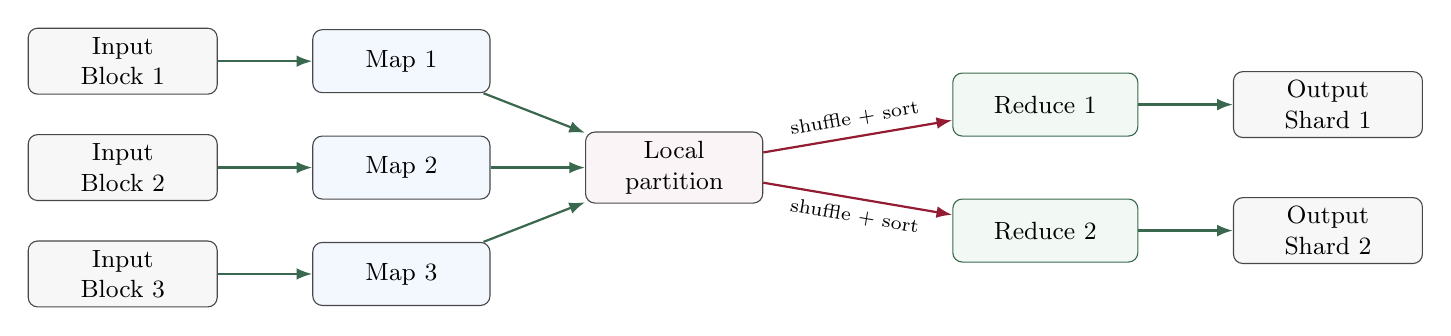
\begin{tikzpicture}[node distance=8mm and 8mm]
\node[storagenode] (b1) {Input\\Block 1};
\node[storagenode, below=5mm of b1] (b2) {Input\\Block 2};
\node[storagenode, below=5mm of b2] (b3) {Input\\Block 3};

\node[mapnode, right=12mm of b1] (m1) {Map 1};
\node[mapnode, right=12mm of b2] (m2) {Map 2};
\node[mapnode, right=12mm of b3] (m3) {Map 3};

\node[mapnode, right=12mm of m2, fill=ShuffleTint] (part) {Local\\partition};

\node[reducernode, right=24mm of part, yshift=8mm] (r1) {Reduce 1};
\node[reducernode, right=24mm of part, yshift=-8mm] (r2) {Reduce 2};

\node[storagenode, right=12mm of r1] (o1) {Output\\Shard 1};
\node[storagenode, right=12mm of r2] (o2) {Output\\Shard 2};

\draw[datarrow] (b1) -- (m1);
\draw[datarrow] (b2) -- (m2);
\draw[datarrow] (b3) -- (m3);

\draw[datarrow] (m1) -- (part);
\draw[datarrow] (m2) -- (part);
\draw[datarrow] (m3) -- (part);

\draw[shufflearrow] (part) -- node[above,sloped,font=\scriptsize]{shuffle + sort} (r1);
\draw[shufflearrow] (part) -- node[below,sloped,font=\scriptsize]{shuffle + sort} (r2);

\draw[datarrow] (r1) -- (o1);
\draw[datarrow] (r2) -- (o2);
\end{tikzpicture}%
}
\caption{MapReduce execution overview: input blocks generate Map tasks; intermediate data is partitioned, shuffled, sorted, and reduced into output shards.}
\label{fig:execution-overview}
\end{figure}

\subsection{Combiners}

\begin{definitionbox}{Combiner}
A combiner is an optional local pre-aggregation step applied to a Map task's output before shuffle, with the goal of reducing the amount of intermediate data transferred across the network.
\end{definitionbox}

For word count, instead of sending many separate \((w,1)\) pairs across the network, a combiner can aggregate them locally.

A combiner may run zero, one, or multiple times, so correctness must not depend on it running exactly once. Local aggregation must preserve the final result under regrouping; associative, commutative operations such as integer addition are suitable. Averages require carrying a sum and count, rather than averaging partial averages.

\subsection{Sharded Output}

Each Reduce task writes its own output file, producing a distributed collection of shards such as

\[
\texttt{part-r-00000},\;
\texttt{part-r-00001},\ldots
\]

rather than one monolithic file. A downstream MapReduce job can then consume these shards as distributed input.

\subsubsection*{Review Questions}
\begin{enumerate}
    \item How do logical input splits relate to physical storage blocks and Map tasks?
    \item How does data locality affect Map-task placement?
    \item What problem does a combiner solve, and where does it run?
    \item What trade-off governs the number of Reduce tasks?
\end{enumerate}


% ============================================================
\section{Shuffle, Sort, and the Reduce Phase}
% ============================================================

\subsection{The Shuffle Phase}

Shuffle transfers intermediate Map output to the correct reducers. Each Reduce task must receive all pairs belonging to its assigned keys, regardless of which Map worker produced them.

This creates an all-to-all communication pattern: every mapper may need to communicate with every reducer.

\begin{definitionbox}{Shuffle}
Shuffle is the distributed transfer of partitioned intermediate data from Map tasks to the Reduce tasks responsible for the corresponding key partitions.
\end{definitionbox}

\subsection{Each Mapper Partitions Its Own Output}

Before network transfer, each Map task applies the partition function to emitted keys. Its local output is divided into \(R\) regions, one per reducer. Reducers later fetch only the regions assigned to them.

\subsection{Why Shuffle Is Expensive}

With \(M\) Map tasks and \(R\) Reduce tasks, the communication pattern can involve up to

\begin{equation}
M\times R
\label{eq:shuffle-links}
\end{equation}

distinct map-to-reduce transfers.

Unlike the Map phase, this traffic generally cannot be made local for every producer--consumer pair.

\begin{figure}[htbp]
\centering
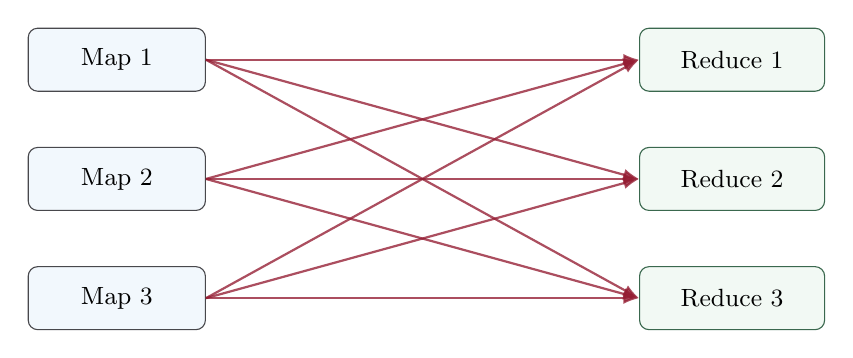
\begin{tikzpicture}[node distance=10mm and 26mm]
\node[mapnode] (m1) {Map 1};
\node[mapnode, below=7mm of m1] (m2) {Map 2};
\node[mapnode, below=7mm of m2] (m3) {Map 3};

\node[reducernode, right=55mm of m1] (r1) {Reduce 1};
\node[reducernode, below=7mm of r1] (r2) {Reduce 2};
\node[reducernode, below=7mm of r2] (r3) {Reduce 3};

\foreach \m in {m1,m2,m3}{
  \foreach \r in {r1,r2,r3}{
    \draw[shufflearrow,opacity=0.78] (\m.east) -- (\r.west);
  }
}
\end{tikzpicture}
\caption{The all-to-all structure of shuffle. Every Map task may contribute data to every Reduce task.}
\label{fig:shuffle-alltoall}
\end{figure}

\subsection{Shuffle Network Volume}

Let \(D\) be the intermediate-data volume after combining and compression. If most partitions are fetched remotely and retries are ignored, shuffle transfers roughly \(D\) bytes over the network. Local fetches reduce network traffic; retries can increase it.

Across \(M R\) logical map-to-reduce pairs, the average partition size is

\begin{equation}
\text{average bytes per map-to-reduce pair}
=
\frac{D}{M R}.
\label{eq:per-link-transfer}
\end{equation}

This is not a worst-case bound or a physical-link bandwidth estimate. Skew can concentrate up to \(D\) bytes in one pair, and a physical network link may carry many pairs. The key contrast is with the Map phase, where input data can often be read locally.

\subsection{Sorting by Intermediate Key}

After a reducer receives its assigned partitions from all mappers, it sorts the data by intermediate key. Sorting places equal keys next to one another and allows the framework to present each reducer invocation with a complete group of values for one key.

\subsection{Why Sorting Simplifies Reduce}

The user-defined Reduce function need not implement its own distributed grouping logic. The framework guarantees that all values for the current key are presented together.

Conceptually, the reducer processes

\[
(k,[v_1,v_2,\ldots,v_n])
\]

one key group at a time.

\begin{keyconcept}
Sorting is not merely an implementation detail: it is the mechanism that turns distributed intermediate records into contiguous key groups with a simple Reduce interface.
\end{keyconcept}

\subsection{Reduce Output}

Final Reduce output is written back to GFS/HDFS, unlike temporary Map output. Each Reduce task creates one output shard, which is then stored and replicated like ordinary distributed-file-system data.

\subsection{Why Shuffle Often Dominates Runtime}

Shuffle combines two expensive resources:

\begin{itemize}
    \item \textbf{network I/O:} all-to-all movement of the intermediate dataset;
    \item \textbf{disk I/O:} Map output is written locally, read back for transfer, and often written or merged again on the Reduce side.
\end{itemize}

For many batch jobs, shuffle rather than user computation is the dominant cost.

\subsection{Mitigating Shuffle Cost}

Two practical techniques reduce this cost:

\begin{itemize}
    \item \textbf{combiners}, which reduce intermediate volume before transfer;
    \item \textbf{compression}, which trades CPU time for reduced network and disk I/O.
\end{itemize}

At cluster scale, this CPU-for-I/O trade can be favourable because network movement is expensive.

% ============================================================
\subsection{End-to-End Word Count Trace}
% ============================================================

Consider:

\[
\text{Doc A}: \texttt{``the cat sat''}
\]

and

\[
\text{Doc B}: \texttt{``the dog ran''}.
\]

The Map phase produces

\[
\operatorname{Map}(\text{Doc A})
\to
(\texttt{the},1),
(\texttt{cat},1),
(\texttt{sat},1),
\]

\[
\operatorname{Map}(\text{Doc B})
\to
(\texttt{the},1),
(\texttt{dog},1),
(\texttt{ran},1).
\]

Assume two reducers and a hash partition in which \(\texttt{the}\) and \(\texttt{cat}\) map to Reduce 1, while \(\texttt{sat}\), \(\texttt{dog}\), and \(\texttt{ran}\) map to Reduce 2.

After shuffle and sort:

\[
R_1:
(\texttt{cat},[1]),
(\texttt{the},[1,1]),
\]

\[
R_2:
(\texttt{dog},[1]),
(\texttt{ran},[1]),
(\texttt{sat},[1]).
\]

Reduce then emits

\[
R_1:
(\texttt{cat},1),
(\texttt{the},2)
\]

and

\[
R_2:
(\texttt{dog},1),
(\texttt{ran},1),
(\texttt{sat},1).
\]

\begin{examplebox}{Why identical keys must share a reducer}
The two occurrences of \texttt{the} originate from different documents and therefore different Map executions, but deterministic partitioning sends both values to the same reducer. Only then can the framework provide the complete group \((\texttt{the},[1,1])\) to one Reduce call.
\end{examplebox}

\subsubsection*{Review Questions}
\begin{enumerate}
    \item Why is shuffle an all-to-all communication pattern?
    \item Why does sorting simplify the Reduce implementation?
    \item Why is shuffle frequently the dominant cost of a MapReduce job?
    \item Why must both occurrences of the same key be routed to the same Reduce task?
\end{enumerate}


% ============================================================
\section{Fault Tolerance and Stragglers}
% ============================================================

\subsection{Computation Introduces New Failure Modes}

Distributed storage must already tolerate disk and node failures. Active computation introduces additional failure modes:

\begin{itemize}
    \item a worker crashes while running a task;
    \item a task remains alive but becomes abnormally slow;
    \item the job coordinator itself fails.
\end{itemize}

\subsection{Worker Failure Detection}

Workers periodically send heartbeats containing liveness and progress information. If a worker misses heartbeats beyond a timeout, the Master marks it as failed and must recover affected work.

\subsection{Failed Map Tasks}

If a Map worker fails, the task is rescheduled on a healthy worker. Even a previously completed Map task may need to be rerun if its intermediate output was stored only on the failed worker's local disk.

The determinism requirement guarantees that rerunning the Map task reconstructs equivalent intermediate output.

\subsection{Failed Reduce Tasks}

A failed Reduce task is also rescheduled, but the recovery path differs. If the necessary Map outputs are still available, the replacement reducer can fetch its partitions again. The original Map computations need not all be repeated.

\begin{table}[htbp]
\centering
\caption{Recovery distinction between failed Map and Reduce tasks.}
\label{tab:map-reduce-failure}
\begin{tabularx}{\textwidth}{>{\bfseries\raggedright\arraybackslash}p{3.0cm} Y Y}
\toprule
\rowcolor{TableTint}
Failure & Recovery & Why \\
\midrule
Map task / worker & Re-execute Map on another worker & Intermediate Map output lived on the failed worker's local disk and may be lost. \\
Reduce task / worker & Re-execute Reduce and re-fetch intermediate partitions & Map outputs can still be fetched from surviving Map workers. \\
\bottomrule
\end{tabularx}
\end{table}

\subsection{Why Re-Execution Is Safe}

Pure deterministic functions make a retry functionally indistinguishable from successful first execution. Without this property, the framework could silently obtain different results after a failure.

\subsection{Idempotency and Atomic Commit}

A subtle case appears when multiple attempts of the same task coexist, either due to retries or speculation. The framework must ensure that only one attempt becomes authoritative.

An atomic-commit pattern addresses this: attempts write to temporary locations, and a coordinated atomic rename or commit makes exactly one result official.

\begin{keyconcept}
Re-execution solves computation failure only if the framework also controls output commitment. Multiple task attempts may run, but only one attempt's output may become the official result.
\end{keyconcept}

\subsection{Master Failure}

The MapReduce Master is itself a point of failure. In the original MapReduce design, Master failure is handled by restarting the entire job.

This is a deliberate simplicity trade-off in Google's original implementation, whose Master coordinates one job. Hadoop v1's JobTracker is a long-lived service managing multiple jobs; YARN separates cluster resource management from a per-application ApplicationMaster.

% ============================================================
\subsection{The Straggler Problem}
% ============================================================

\begin{definitionbox}{Straggler}
A straggler is a task that remains alive and responsive but executes much more slowly than comparable tasks, thereby delaying overall job completion.
\end{definitionbox}

Heartbeats do not classify a straggler as failed because the worker is still responding. If \(999\) tasks finish quickly and one task takes much longer, the entire job still waits for the slowest task.

\subsection{Causes of Stragglers}

Common causes include:

\begin{itemize}
    \item hardware degradation;
    \item CPU, disk, or network contention;
    \item data skew, especially when one reducer receives an unusually large key group.
\end{itemize}

% ============================================================
\subsection{Speculative Execution}
% ============================================================

\begin{definitionbox}{Speculative Execution}
Speculative execution launches a backup copy of an unusually slow task on another available worker. The first attempt to finish becomes the accepted result, and the slower copy is discarded.
\end{definitionbox}

Near the end of a job, the Master identifies tasks running significantly slower than their peers and launches backup attempts if spare cluster capacity exists.

\begin{figure}[htbp]
\centering
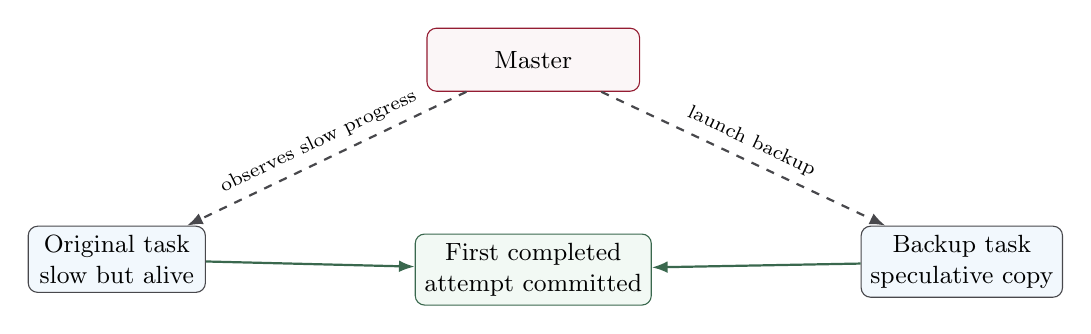
\begin{tikzpicture}[node distance=13mm and 19mm]
\node[masternode] (m) {Master};
\node[mapnode, below left=17mm and 28mm of m] (orig) {Original task\\slow but alive};
\node[mapnode, below right=17mm and 28mm of m] (backup) {Backup task\\speculative copy};
\node[reducernode, below=18mm of m] (commit) {First completed\\attempt committed};

\draw[ctrlarrow] (m) -- node[above,sloped,font=\scriptsize]{observes slow progress} (orig);
\draw[ctrlarrow] (m) -- node[above,sloped,font=\scriptsize]{launch backup} (backup);
\draw[datarrow] (orig) -- (commit);
\draw[datarrow] (backup) -- (commit);
\end{tikzpicture}
\caption{Speculative execution: the runtime duplicates a slow task and accepts the first successful attempt.}
\label{fig:speculative-execution}
\end{figure}

\subsection{Numeric Example}

Suppose a Map stage has \(1000\) tasks, enough slots to start them together, and spare capacity for a backup. Normal tasks take approximately \(10\) seconds, but one straggler takes \(200\) seconds. Assume the backup starts at \(t=10\) seconds and takes another \(10\) seconds; ignore scheduling and commit overhead.

\begin{table}[htbp]
\centering
\caption{Illustrative effect of speculative execution on completion time.}
\label{tab:speculation-example}
\begin{tabularx}{0.78\textwidth}{>{\bfseries\raggedright\arraybackslash}p{4.2cm} Y}
\toprule
\rowcolor{TableTint}
Scenario & Approximate Map-stage completion time \\
\midrule
Without speculation & \(\sim 200\) s, bounded by the straggler \\
With speculation & \(\sim 20\) s: backup starts at \(10\) s and runs for \(10\) s \\
\bottomrule
\end{tabularx}
\end{table}

The example illustrates that a single straggler can dominate job completion time even when almost all other work has finished.

\subsection{Speculation Trade-off}

Speculation is not free:

\begin{itemize}
    \item \textbf{benefit:} it can sharply reduce tail completion time when only a small number of tasks are anomalously slow;
    \item \textbf{cost:} backup attempts consume resources even though one attempt will eventually be discarded.
\end{itemize}

Speculation is therefore triggered selectively for sufficiently slow tasks when spare capacity is available.

\subsubsection*{Review Questions}
\begin{enumerate}
    \item Why is re-execution of a failed Map task safe?
    \item What is the key difference between recovery from a failed Map task and a failed Reduce task?
    \item Why do heartbeat timeouts not detect stragglers?
    \item How does speculative execution work, and what is its principal cost?
\end{enumerate}


% ============================================================
\section{Synthesis}
% ============================================================

\subsection{Full MapReduce Pipeline}

\begin{figure}[htbp]
\centering
\resizebox{0.96\textwidth}{!}{%
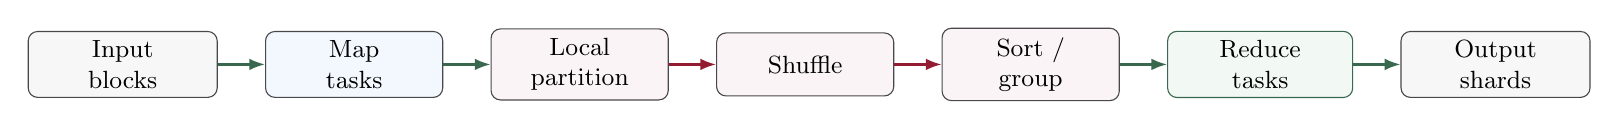
\begin{tikzpicture}[node distance=6mm]
\node[storagenode] (in) {Input\\blocks};
\node[mapnode, right=of in] (map) {Map\\tasks};
\node[mapnode, right=of map, fill=ShuffleTint] (part) {Local\\partition};
\node[mapnode, right=of part, fill=ShuffleTint] (shuffle) {Shuffle};
\node[mapnode, right=of shuffle, fill=ShuffleTint] (sort) {Sort /\\group};
\node[reducernode, right=of sort] (red) {Reduce\\tasks};
\node[storagenode, right=of red] (out) {Output\\shards};

\draw[datarrow] (in) -- (map);
\draw[datarrow] (map) -- (part);
\draw[shufflearrow] (part) -- (shuffle);
\draw[shufflearrow] (shuffle) -- (sort);
\draw[datarrow] (sort) -- (red);
\draw[datarrow] (red) -- (out);
\end{tikzpicture}%
}
\caption{Complete MapReduce pipeline from distributed input blocks to distributed output shards.}
\label{fig:full-pipeline}
\end{figure}

The execution model can be read as a sequence:

\[
\text{input blocks}
\rightarrow
\text{Map}
\rightarrow
\text{local partition}
\rightarrow
\text{shuffle}
\rightarrow
\text{sort/group}
\rightarrow
\text{Reduce}
\rightarrow
\text{output}.
\]

Fault tolerance surrounds this pipeline through worker heartbeats, re-execution, output commit control, and speculative execution.

\subsection{Storage versus Compute Layer}

\begin{table}[htbp]
\centering
\caption{Comparison between the storage and computation layers.}
\label{tab:storage-compute}
\begin{tabularx}{\textwidth}{>{\bfseries\raggedright\arraybackslash}p{3.1cm} Y Y}
\toprule
\rowcolor{TableTint}
Aspect & Storage Layer & Compute Layer \\
\midrule
Coordinator & Master / NameNode & Master / JobTracker \\
Worker unit & Chunkserver / DataNode & Map / Reduce task on workers \\
Failure detection & Heartbeats & Heartbeats \\
Recovery strategy & Re-replication & Re-execution \\
New mechanism & -- & Speculative execution for stragglers \\
\bottomrule
\end{tabularx}
\end{table}

The two layers share a philosophy: centralized coordination, many workers, heartbeat-based detection, and automatic recovery. Their recovery operations differ because storage reconstructs replicas, while computation reconstructs work.

\subsection{Strengths of MapReduce}

The model's strengths include:

\begin{itemize}
    \item \textbf{simplicity:} programmers define two sequential-looking functions;
    \item \textbf{built-in fault tolerance:} deterministic tasks can be transparently retried;
    \item \textbf{data locality:} Map scheduling exploits block placement from GFS/HDFS;
    \item \textbf{generality:} many batch-processing tasks can be expressed through the model.
\end{itemize}

\subsection{Limitations}

The same design choices introduce important limitations.

\begin{itemize}
    \item \textbf{Disk-heavy execution:} intermediate data is materialized on disk between Map and Reduce.
    \item \textbf{Rigid two-stage structure:} complex workflows require chaining multiple jobs.
    \item \textbf{Repeated shuffle cost:} each chained job pays another partition/shuffle/sort overhead.
    \item \textbf{High latency:} the model is optimized for batch throughput rather than interactive response.
\end{itemize}

These limitations motivate in-memory DAG execution models such as Apache Spark.

\subsection{Iterative Pipelines}

Consider a pipeline of ten successive MapReduce jobs in which each job's output feeds the next. Such a workload repeatedly materializes intermediate data and repeatedly pays shuffle and disk-I/O costs.

This motivates retaining reusable intermediate state in memory and scheduling a more general computation graph, avoiding repeated materialization costs in later in-memory execution systems.

% ============================================================
\section{Key Terms}
% ============================================================

\begin{table}[htbp]
\centering
\caption{Key MapReduce terminology.}
\label{tab:mapreduce-key-terms}
\begin{tabularx}{\textwidth}{>{\bfseries\raggedright\arraybackslash}p{4.1cm} Y}
\toprule
Term & Meaning \\
\midrule
Map task & Processes one input split and emits intermediate \((key,value)\) pairs. \\
Reduce task & Processes grouped values for its assigned intermediate-key partition. \\
Partition function & Maps an intermediate key to one Reduce task. \\
Shuffle & Transfers partitioned intermediate data from Map workers to Reduce workers. \\
Sort / group & Organizes intermediate records so that all values of one key are contiguous. \\
Combiner & Performs optional local pre-aggregation before shuffle. \\
Straggler & Task that remains alive but runs abnormally slowly. \\
Speculative execution & Runs a backup copy of a slow task on another worker and uses the first completed attempt. \\
Re-execution & Runs a failed task again on a healthy worker. \\
Atomic commit & Ensures only one concurrent task attempt becomes the official output. \\
Data locality & Schedules Map computation near its distributed input block. \\
Output shard & One output file produced by a Reduce task. \\
\bottomrule
\end{tabularx}
\end{table}

% ============================================================
\section{Chapter Summary}
% ============================================================

\begin{longtable}{>{\bfseries\raggedright\arraybackslash}p{\dimexpr0.25\textwidth-2\tabcolsep\relax} >{\raggedright\arraybackslash}p{\dimexpr0.355\textwidth-2\tabcolsep\relax} >{\raggedright\arraybackslash}p{\dimexpr0.395\textwidth-2\tabcolsep\relax}}
\caption{Compact summary of the main relationships in the MapReduce execution model.}
\label{tab:mapreduce-core-summary}\\
\toprule
Concept & Main role & Key relationship / trade-off \\
\midrule
\endfirsthead
\toprule
Concept & Main role & Key relationship / trade-off \\
\midrule
\endhead
Map & Transform independent input records & Stateless independence enables arbitrary parallel scheduling. \\
Reduce & Aggregate all values for one key & Framework-provided grouping hides distributed aggregation mechanics. \\
Determinism & Make retries reproduce the same logical result & Enables transparent re-execution after failure. \\
Input block & Natural Map split & Connects distributed storage directly to computation parallelism. \\
Data locality & Place Maps near their inputs & Minimizes network traffic in the Map phase. \\
Local Map output & Temporary intermediate storage & Avoids unnecessary DFS replication, but is lost if the worker fails. \\
Hash partitioning & Route equal keys to one reducer & Deterministic mapping ensures complete key groups. \\
Number of reducers & Control Reduce parallelism & Too few reducers limit parallelism; too many create coordination and output overhead. \\
Combiner & Pre-aggregate locally & Reduces shuffle volume when local combination is valid. \\
Shuffle & Move partitions from Maps to Reducers & All-to-all traffic makes network and disk I/O expensive. \\
Sort & Group equal keys contiguously & Simplifies the Reduce interface. \\
Failed Map & Re-execute task & Lost local intermediate output must be regenerated. \\
Failed Reduce & Re-execute and re-fetch & Existing Map output can generally be fetched again. \\
Atomic commit & Select one authoritative attempt & Protects output correctness when multiple attempts coexist. \\
Straggler & Slow but alive task & Not detected as failure because heartbeats continue. \\
Speculative execution & Duplicate slow work & Reduces tail latency at the cost of extra resources. \\
Master failure & Job-level coordinator failure & Original design favors restarting the job for simplicity. \\
MapReduce strength & Simple resilient batch abstraction & Hides distribution and failure handling. \\
MapReduce limitation & Disk-heavy two-stage model & Iterative pipelines repeatedly pay materialization and shuffle costs. \\
Spark motivation & General in-memory DAG execution & Addresses rigidity and repeated disk/shuffle overhead. \\
\bottomrule
\end{longtable}

% ============================================================
\section{Quick Review}
% ============================================================

\begin{enumerate}
    \item MapReduce turns simple Map and Reduce functions into distributed computations managed by a runtime.
    \item Map processes one input record independently and may emit zero, one, or many intermediate pairs.
    \item Reduce receives one intermediate key and the complete collection of values associated with that key.
    \item The runtime, not the programmer, handles scheduling, networking, grouping, retry logic, and worker placement.
    \item Deterministic, side-effect-free tasks make transparent re-execution safe.
    \item Word count Maps words to \((word,1)\) pairs and Reduce sums the values per word.
    \item An inverted index uses the same execution structure with different intermediate values and aggregation.
    \item Input blocks from GFS/HDFS naturally become units of Map parallelism.
    \item Map tasks are scheduled with data locality whenever possible.
    \item The number of Map tasks is commonly much larger than the number of machines, so tasks execute in waves.
    \item Intermediate Map output is stored locally rather than immediately replicated into the distributed file system.
    \item Hash partitioning uses \(\operatorname{hash}(key)\bmod R\) to route identical keys deterministically to the same reducer.
    \item The number of Reduce tasks controls the balance between parallelism and coordination/output overhead.
    \item A combiner performs optional local pre-aggregation and can reduce shuffle traffic.
    \item Shuffle is an all-to-all pattern in which each mapper may send data to every reducer.
    \item With \(M\) mappers and \(R\) reducers, the shuffle can involve up to \(M\times R\) logical transfers.
    \item Shuffle often dominates runtime because it combines network transfer with repeated disk I/O.
    \item Sorting groups identical keys so the Reduce function receives one complete value collection at a time.
    \item Final Reduce output is written back to GFS/HDFS as sharded output files.
    \item Failed Map tasks are rerun because their local intermediate output may be lost with the failed worker.
    \item Failed Reduce tasks can be rerun and normally re-fetch existing Map outputs.
    \item Atomic commit prevents multiple concurrent attempts of the same task from producing multiple official outputs.
    \item A straggler is slow but alive, so heartbeat-based failure detection does not classify it as failed.
    \item Speculative execution launches backup attempts for slow tasks and accepts whichever attempt finishes first.
    \item Speculation reduces tail latency but consumes additional cluster resources.
    \item MapReduce's major limitations are disk-heavy execution, rigid two-stage jobs, repeated shuffle cost, and high batch latency.
    \item These limitations motivate the in-memory DAG model used by Apache Spark.
\end{enumerate}

% ============================================================
\section{Further Reading}
% ============================================================

Further reading includes:

\begin{itemize}
    \item Dean, J., \& Ghemawat, S. (2004). \href{https://research.google.com/archive/mapreduce-osdi04.pdf}{\emph{MapReduce: Simplified Data Processing on Large Clusters}}. OSDI. A later version appeared in \emph{Communications of the ACM}, 51(1), in 2008.
    \item Apache Hadoop. \href{https://hadoop.apache.org/docs/r3.3.3/hadoop-mapreduce-client/hadoop-mapreduce-client-core/MapReduceTutorial.html}{\emph{MapReduce Tutorial}}, including input splits, shuffle, and output commitment.
\end{itemize}


% ============================================================
\chapter[Apache Spark and Dataflow Graph Architectures]{Apache Spark and Dataflow Graph\\Architectures}
\label{chap:spark-dag}
% ============================================================

MapReduce established that large distributed computations can survive routine worker failures through deterministic re-execution, but its execution model remains deliberately rigid and disk-oriented. Spark preserves the recoverability principle while changing the cost model: reusable intermediate state can remain in memory, computation is expressed as a general directed acyclic graph (DAG), and lost data can be reconstructed from recorded lineage instead of replicating every intermediate result.

This chapter develops the model through seven linked ideas: the limitations of chained MapReduce jobs, Resilient Distributed Datasets (RDDs), transformations and actions, lazy evaluation and execution DAGs, narrow versus wide dependencies, lineage-based fault tolerance, and the role of the DAG scheduler in turning a logical plan into physical stages and tasks.

\begin{keyconcept}
Spark generalizes MapReduce from a fixed two-stage, disk-heavy job into an arbitrary DAG of operations. Its central performance mechanism is reuse of in-memory data; its central recovery mechanism is lineage-based recomputation.
\end{keyconcept}

% ============================================================
\section{Beyond Two-Stage Pipelines}
\label{sec:spark-beyond-mapreduce}
% ============================================================

\subsection{The MapReduce Ceiling Revisited}

Chapter~\ref{chap:scale-out-storage} established the storage substrate, while Chapter~2 showed how MapReduce executes reliable batch computations on top of it. The same MapReduce design choices that make the model simple also create three limitations for more complex workloads:

\begin{itemize}
    \item \textbf{Disk-heavy execution:} intermediate results are materialized between jobs, so repeated pipelines repeatedly pay storage I/O.
    \item \textbf{Rigid two-stage structure:} each job has the fixed Map $\rightarrow$ Shuffle/Sort $\rightarrow$ Reduce shape.
    \item \textbf{High latency for iterative or interactive work:} each additional job incurs scheduling, materialization, and data-transfer overhead.
\end{itemize}

Spark was introduced through the Resilient Distributed Datasets paper by Zaharia et al. (NSDI 2012) specifically to improve data reuse across multiple operations and iterations.

\subsection{Why Chaining MapReduce Jobs Is Expensive}

A real analytics workflow may need filtering, transformations, joins, aggregation, and further filtering. Under the classic MapReduce model, a multi-step computation is represented as a sequence of independent jobs:

\begin{center}
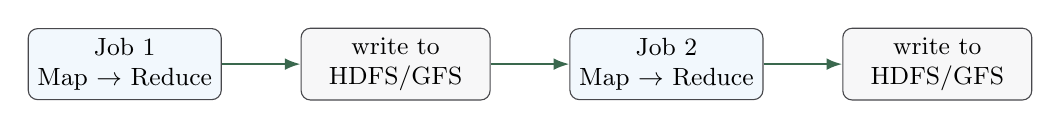
\begin{tikzpicture}[node distance=10mm]
\node[mapnode] (j1) {Job 1\\Map $\rightarrow$ Reduce};
\node[storagenode, right=of j1] (h1) {write to\\HDFS/GFS};
\node[mapnode, right=of h1] (j2) {Job 2\\Map $\rightarrow$ Reduce};
\node[storagenode, right=of j2] (h2) {write to\\HDFS/GFS};
\draw[datarrow] (j1) -- (h1);
\draw[datarrow] (h1) -- (j2);
\draw[datarrow] (j2) -- (h2);
\end{tikzpicture}
\end{center}

Each job is scheduled and torn down independently. Its complete output is written to the distributed file system and must be read again by the next job. In a ten-stage iterative pipeline, the motivating ten-stage example therefore pays ten full disk round-trips and ten shuffle phases even though only the initial input and final output truly require durable storage.

\subsection{Arbitrary Computation Graphs}

The natural structure of a multi-operation program is not a fixed two-stage pipeline but a graph of data dependencies. A \textbf{Directed Acyclic Graph (DAG)} represents this structure:

\begin{itemize}
    \item nodes represent operations or the datasets those operations produce;
    \item directed edges represent dependencies between producers and consumers;
    \item acyclicity means execution flows forward through the dependency graph rather than forming a cyclic dependency.
\end{itemize}

A MapReduce job can be viewed as a very restricted DAG. Spark removes that restriction and allows the programmer to express arbitrary chains and branches of operations.

\begin{figure}[htbp]
\centering
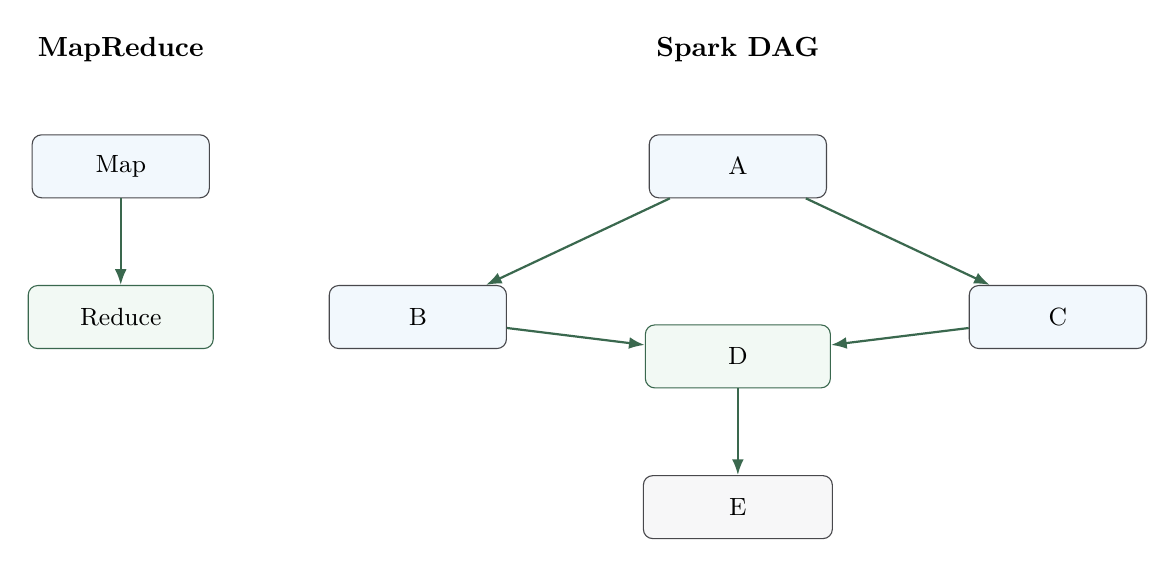
\begin{tikzpicture}[node distance=11mm and 18mm]
% left: fixed MapReduce
\node[font=\bfseries] (lhead) {MapReduce};
\node[mapnode, below=8mm of lhead] (m) {Map};
\node[reducernode, below=of m] (r) {Reduce};
\draw[datarrow] (m) -- (r);
% right: DAG
\node[font=\bfseries, right=55mm of lhead] (rhead) {Spark DAG};
\node[mapnode, below=8mm of rhead] (a) {A};
\node[mapnode, below left=of a] (b) {B};
\node[mapnode, below right=of a] (c) {C};
\node[reducernode, below=16mm of a] (d) {D};
\node[storagenode, below=of d] (e) {E};
\draw[datarrow] (a) -- (b);
\draw[datarrow] (a) -- (c);
\draw[datarrow] (b) -- (d);
\draw[datarrow] (c) -- (d);
\draw[datarrow] (d) -- (e);
\end{tikzpicture}
\caption{A fixed MapReduce pipeline compared with an arbitrary Spark computation DAG. Spark can represent branches, joins, and deeper operation chains rather than exactly one Map and one Reduce phase.}
\label{fig:spark-dag-vs-mapreduce}
\end{figure}

\subsection{What ``Memory-Centric'' Means}

Spark's second major shift is that intermediate results can remain in RAM across operations rather than being written to durable storage after every step. Data is written to durable storage when explicitly requested or when memory pressure requires another storage strategy.

The memory hierarchy discussed in Chapter~\ref{chap:scale-out-storage} provides the performance intuition: RAM access is roughly two orders of magnitude faster than disk access for comparable data volumes. Reusing an in-memory working set is therefore especially valuable when an algorithm repeatedly scans the same dataset.

\subsection{Motivating Workloads}

Two workload classes motivate the design particularly strongly.

\textbf{Iterative algorithms.} Graph algorithms and machine-learning training loops repeatedly process the same data. In MapReduce, every iteration can require another full job, another read, and another materialization. Spark can retain the working dataset across iterations.

\textbf{Interactive and exploratory analysis.} An analyst may issue multiple successive queries over the same dataset. Once that dataset is cached in cluster memory, later queries can avoid repeated disk I/O and complete much more quickly than a fresh batch job that reloads the same input every time.

\subsection{MapReduce and Spark Side by Side}

\begin{table}[htbp]
\centering
\caption{Positioning Spark relative to the MapReduce execution model.}
\label{tab:mapreduce-spark-positioning}
\begin{tabularx}{\textwidth}{>{\bfseries\raggedright\arraybackslash}p{3.2cm} Y Y}
\toprule
\rowcolor{TableTint}
Aspect & MapReduce & Spark \\
\midrule
Pipeline shape & Fixed two-stage Map $\rightarrow$ Reduce model & Arbitrary DAG of operations \\
Intermediate data & Materialized to disk between chained jobs & Held in memory when possible \\
Reuse across iterations & Re-read or recomputed through separate jobs & Cached in memory across iterations \\
Fault tolerance & Re-execution of failed tasks & Lineage-based recomputation of lost partitions \\
Best fit in this comparison & Large, one-pass batch jobs & Iterative, interactive, and multi-step pipelines \\
\bottomrule
\end{tabularx}
\end{table}

\subsubsection*{Review Questions}
\begin{enumerate}
    \item What three limitations of MapReduce does Spark directly address?
    \item Why is chaining multiple MapReduce jobs expensive even when each individual job is efficient?
    \item How does a DAG generalize the fixed two-stage MapReduce pipeline?
    \item Why do iterative algorithms benefit disproportionately from memory-centric execution?
\end{enumerate}

% ============================================================
\section{Resilient Distributed Datasets}
\label{sec:rdds}
% ============================================================

\subsection{RDD as the Core Abstraction}

\begin{definitionbox}{Resilient Distributed Dataset (RDD)}
An RDD is an immutable collection of elements partitioned across the machines of a cluster. It is resilient because lost partitions can be reconstructed automatically from the recorded derivation history rather than requiring every intermediate dataset to be physically replicated.
\end{definitionbox}

An RDD behaves conceptually like a large distributed collection. Within the RDD programming model used here, every dataset manipulated by the Spark program is represented through this abstraction. Operations derive new RDDs from existing ones; an existing RDD is never modified in place. This intentionally hides much of the cluster-level complexity from the programmer.

\subsection{Why Immutability Matters}

Immutability is foundational rather than cosmetic. Because an RDD never changes after creation, the transformation that created it remains a complete and permanent description of how its contents can be reconstructed. This property supports lineage-based fault tolerance and also avoids many concurrency problems associated with shared mutable state distributed across machines.

\begin{keyconcept}
For an immutable RDD, ``how this dataset was created'' is stable metadata. Spark can therefore retain the recipe for an intermediate dataset instead of maintaining a replicated physical copy of that dataset at all times.
\end{keyconcept}

\subsection{Partitions: The Unit of Parallelism}

RDDs are divided into \textbf{partitions}. Each partition contains a subset of the RDD's data and can be processed independently by a task. Consequently, the partition count bounds the maximum degree of parallelism available for operations on that RDD.

\begin{figure}[htbp]
\centering
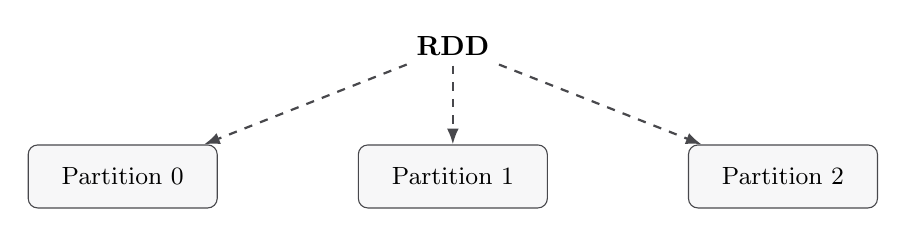
\begin{tikzpicture}[node distance=8mm and 10mm]
\node[font=\bfseries] (rdd) {RDD};
\node[storagenode, below left=10mm and 24mm of rdd] (p0) {Partition 0};
\node[storagenode, below=10mm of rdd] (p1) {Partition 1};
\node[storagenode, below right=10mm and 24mm of rdd] (p2) {Partition 2};
\draw[ctrlarrow] (rdd) -- (p0);
\draw[ctrlarrow] (rdd) -- (p1);
\draw[ctrlarrow] (rdd) -- (p2);
\end{tikzpicture}
\caption{An RDD is logically one dataset but is physically processed as independent partitions distributed across the cluster.}
\label{fig:rdd-partitions}
\end{figure}

\subsection{RDD Partitions versus Storage Blocks}

RDD partitions are related to, but distinct from, the GFS/HDFS blocks studied in Chapter~\ref{chap:scale-out-storage}. If an RDD is created from a distributed file, its partitions commonly correspond to underlying file blocks. However, an RDD can also be repartitioned explicitly or created from a non-file source such as an in-memory collection. Partitioning is therefore a computational concept at the RDD layer rather than a property tied permanently to one storage layout.

\subsection{RDDs and Underlying Storage}

An RDD is not a storage system. It is a computation abstraction layered on top of storage. Its initial data may come from HDFS, GFS, another backend, or a collection in the driver program that is distributed to the cluster.

Two primary RDD-creation patterns are:

\begin{lstlisting}[style=sparkcode]
# From distributed storage
rdd = sc.textFile("hdfs://path/to/data")

# From an existing in-memory collection
rdd = sc.parallelize([1, 2, 3, 4, 5])
\end{lstlisting}

With \texttt{textFile}, partitions are derived from the underlying file organization. With \texttt{parallelize}, the driver's local collection is divided into partitions and distributed.

\subsection{Logical Handle versus Materialized Data}

An RDD should be understood as a \emph{logical handle}: it describes a dataset, its partitioning, and the computation from which it is derived. The corresponding bytes do not necessarily exist in memory at the moment the RDD variable is created. Materialization depends on lazy evaluation and on whether the program chooses to cache the RDD.

\subsection{The ``Resilient'' Property}

Unlike GFS/HDFS, resilience for an intermediate RDD does not normally come from keeping several copies of every partition. Spark records the RDD's \textbf{lineage}: which parent RDD or RDDs it depends on and which transformation produced it. If a partition disappears because a worker fails, Spark can recompute that partition from its lineage.

\subsection{RDD Interface Overview}

The RDD interface exposes three families of operations:

\begin{itemize}
    \item \textbf{Transformations}, which derive new RDDs from existing RDDs;
    \item \textbf{Actions}, which trigger computation and return a result to the driver or write output;
    \item \textbf{Persistence controls}, which request that computed partitions be retained for reuse.
\end{itemize}

This generalizes the MapReduce input model. An RDD can begin from storage blocks just as MapReduce begins from distributed input, but it can then pass through an arbitrary sequence of transformations instead of being restricted to one Map phase and one Reduce phase.

\subsection{RDDs versus Regular Distributed Arrays}

An RDD resembles a distributed array or list, but three properties distinguish it in this model:

\begin{itemize}
    \item there are no random in-place updates to individual elements;
    \item the system tracks lineage describing how the RDD was produced;
    \item materialization is lazy, so the contents may not exist physically until an action requires them.
\end{itemize}

\subsection{Caching and Persistence}

Caching is the performance mechanism that turns an RDD from a recomputable logical description into a reusable in-memory working set.

\begin{lstlisting}[style=sparkcode]
rdd = sc.textFile("hdfs://path/to/data")
rdd.cache()       # mark the RDD for in-memory persistence
\end{lstlisting}

Without caching, an RDD may be recomputed from lineage when it is reused. With caching, computed partitions are retained and can be consumed directly by later operations, which is especially useful for iterative and interactive workloads.

\begin{table}[htbp]
\centering
\caption{Common RDD persistence levels.}
\label{tab:rdd-persistence-levels}
\begin{tabularx}{0.92\textwidth}{>{\bfseries\raggedright\arraybackslash}p{3.3cm} Y}
\toprule
\rowcolor{TableTint}
Storage level & Behaviour \\
\midrule
Memory only & Fastest; partitions that do not fit are discarded and recomputed when needed. \\
Memory and disk & Keeps partitions in memory when possible and spills excess partitions to local disk. \\
Disk only & Avoids memory pressure but accesses persisted partitions at disk speed. \\
\bottomrule
\end{tabularx}
\end{table}

The appropriate persistence level depends on the size of the working dataset relative to available cluster memory.

\subsubsection*{Review Questions}
\begin{enumerate}
    \item What does it mean for an RDD to be immutable, and why does this matter for fault tolerance?
    \item How do RDD partitions relate to, but differ from, the storage blocks studied in Chapter~\ref{chap:scale-out-storage}?
    \item Why is RDD fault tolerance fundamentally different from GFS/HDFS replication?
    \item What is the purpose of explicitly caching an RDD?
\end{enumerate}

% ============================================================
\section{Transformations and Actions}
\label{sec:spark-transformations-actions}
% ============================================================

\subsection{Two Categories of RDD Operations}

Every RDD operation considered here belongs to one of two categories.

\begin{definitionbox}{Transformation}
A transformation takes one or more RDDs and returns a new RDD describing a derived dataset. The transformation is recorded lazily rather than executed immediately.
\end{definitionbox}

\begin{definitionbox}{Action}
An action triggers the computation needed to produce a result outside the RDD abstraction, either by returning data to the driver program or by writing output to storage.
\end{definitionbox}

This division between \emph{describing} computation and \emph{triggering} computation is the foundation of Spark's lazy evaluation model.

\subsection{Common Transformations}

\begin{table}[htbp]
\centering
\caption{Common RDD transformations.}
\label{tab:spark-transformations}
\begin{tabularx}{0.82\textwidth}{>{\ttfamily\raggedright\arraybackslash}p{3.2cm} Y}
\toprule
\rowcolor{TableTint}
\normalfont\bfseries Transformation & \normalfont\bfseries Effect \\
\midrule
map(f) & Apply \texttt{f} to each element. \\
filter(f) & Keep elements for which \texttt{f} returns true. \\
flatMap(f) & Apply \texttt{f} and flatten the produced collections. \\
distinct() & Remove duplicate elements. \\
union(other) & Combine with another RDD. \\
groupByKey() & Group values by key. \\
reduceByKey(f) & Aggregate values per key using \texttt{f}. \\
join(other) & Join two key-value RDDs by key. \\
\bottomrule
\end{tabularx}
\end{table}

These transformations are deterministic functions over data, analogous in spirit to the deterministic Map operation studied in Chapter~2. Because RDDs are immutable, a transformation does not alter its input:

\begin{lstlisting}[style=sparkcode]
rdd1 = sc.textFile("data.txt")
rdd2 = rdd1.filter(lambda line: "error" in line)
# rdd1 is unchanged; rdd2 is a new RDD description
\end{lstlisting}

A chain of transformations therefore constructs a chain of new RDD descriptions.

\subsection{Common Actions}

\begin{table}[htbp]
\centering
\caption{Common RDD actions.}
\label{tab:spark-actions}
\begin{tabularx}{0.82\textwidth}{>{\ttfamily\raggedright\arraybackslash}p{4.1cm} Y}
\toprule
\rowcolor{TableTint}
\normalfont\bfseries Action & \normalfont\bfseries Effect \\
\midrule
count() & Return the number of elements. \\
collect() & Return all elements to the driver. \\
take(n) & Return the first \texttt{n} elements. \\
reduce(f) & Aggregate all elements using \texttt{f}. \\
saveAsTextFile(path) & Write the RDD contents to storage. \\
\bottomrule
\end{tabularx}
\end{table}

Calling a transformation records another step in the plan. Calling an action forces Spark to execute the transformations required to obtain that action's result.

\subsection{Worked Example: Word Count with RDDs}

The MapReduce word-count example can be rewritten as a chain of RDD transformations:

\begin{lstlisting}[style=sparkcode]
lines  = sc.textFile("hdfs://documents/")
words  = lines.flatMap(lambda line: line.split())
pairs  = words.map(lambda word: (word, 1))
counts = pairs.reduceByKey(lambda a, b: a + b)
\end{lstlisting}

At this point, \texttt{lines}, \texttt{words}, \texttt{pairs}, and \texttt{counts} are logical RDD descriptions. No HDFS input necessarily has been read yet, and no word counting has happened.

Execution starts when an action is called:

\begin{lstlisting}[style=sparkcode]
result = counts.collect()   # ACTION: triggers the entire chain
\end{lstlisting}

This one action causes Spark to read the input, run \texttt{flatMap}, run \texttt{map}, perform \texttt{reduceByKey} including any required shuffle, and return the final result to the driver.

\begin{keyconcept}
Transformations are not ``free.'' Their execution cost is deferred until an action. Laziness changes \emph{when} work happens and gives Spark visibility over the entire transformation chain before deciding how to execute it.
\end{keyconcept}

\subsection{Why the Split Creates an Optimization Opportunity}

If every transformation executed eagerly when called, the system would optimize operations one at a time. By delaying execution, Spark can inspect the complete chain and reason about the pipeline as a whole before physical work begins.

\begin{table}[htbp]
\centering
\caption{MapReduce's eager job model and Spark's lazy RDD model.}
\label{tab:eager-vs-lazy}
\begin{tabularx}{\textwidth}{>{\bfseries\raggedright\arraybackslash}p{3.5cm} Y Y}
\toprule
\rowcolor{TableTint}
Aspect & MapReduce & Spark RDDs \\
\midrule
When work happens & As each submitted job executes & Deferred until an action is called \\
Pipeline visibility & One job at a time & Entire transformation chain visible before execution \\
Multiple steps & Separate jobs with separate materialization & One logical chain that can be optimized and executed together \\
\bottomrule
\end{tabularx}
\end{table}

\subsubsection*{Review Questions}
\begin{enumerate}
    \item What is the fundamental difference between a transformation and an action?
    \item In the word-count example, why has no actual computation happened until \texttt{collect()} is called?
    \item Why does separating the description of computation from its execution create an optimization opportunity?
    \item Give one transformation and one action that do not appear in the word-count chain.
\end{enumerate}

% ============================================================
\section{Lazy Evaluation and the Execution DAG}
\label{sec:spark-lazy-dag}
% ============================================================

\subsection{What Laziness Means}

Lazy evaluation means that transformations update Spark's internal computation plan rather than immediately reading, transforming, or writing partitions. An action is the event that forces execution of the required part of that plan.

This delay has two direct benefits:

\begin{itemize}
    \item Spark can optimize across the entire sequence of transformations rather than executing each step in isolation.
    \item Spark can sometimes avoid work that is irrelevant to the requested result, for example when an action such as \texttt{take(5)} requires only part of the dataset.
\end{itemize}

\subsection{Building the Logical Execution Plan}

Each derived RDD stores references to its parent RDD or RDDs and to the transformation that produced it. These references form a graph. In the simple word-count case the graph is a chain; operations such as \texttt{join} or \texttt{union} can create nodes with multiple incoming dependencies.

\begin{figure}[htbp]
\centering
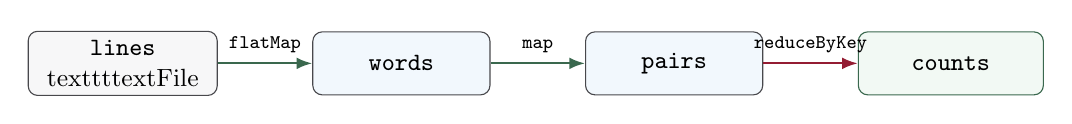
\begin{tikzpicture}[node distance=12mm]
\node[storagenode] (lines) {\texttt{lines}\\texttt{textFile}};
\node[mapnode, right=of lines] (words) {\texttt{words}};
\node[mapnode, right=of words] (pairs) {\texttt{pairs}};
\node[reducernode, right=of pairs] (counts) {\texttt{counts}};
\draw[datarrow] (lines) -- node[above,font=\scriptsize]{\texttt{flatMap}} (words);
\draw[datarrow] (words) -- node[above,font=\scriptsize]{\texttt{map}} (pairs);
\draw[shufflearrow] (pairs) -- node[above,font=\scriptsize]{\texttt{reduceByKey}} (counts);
\end{tikzpicture}
\caption{Logical RDD DAG for the word-count chain. The nodes are RDDs and the edges are transformations. The graph exists before \texttt{collect()} triggers physical execution.}
\label{fig:wordcount-logical-dag}
\end{figure}

\subsection{Optimization Opportunities Enabled by Laziness}

With the full DAG available before execution, Spark can exploit several optimization opportunities:

\begin{itemize}
    \item \textbf{Operator fusion / pipelining:} compatible operations are applied in one pass without materializing complete intermediate datasets.
    \item \textbf{Avoiding unneeded computation:} parts of the DAG that do not contribute to the requested action can sometimes be skipped.
    \item \textbf{Choosing a physical execution structure:} the dependency graph determines where the logical chain must be broken into separate stages.
\end{itemize}

\subsection{Operator Fusion within a Stage}

Consider a narrow chain such as:

\begin{lstlisting}[style=sparkcode]
words.map(f).filter(g).map(h)
\end{lstlisting}

Spark can apply \texttt{f}, then \texttt{g}, then \texttt{h} to each element in one per-partition pass rather than fully materializing the output of each operation. This reduces extra scans and unnecessary intermediate memory usage.

The contrast with chained MapReduce jobs is fundamental: a MapReduce job boundary requires complete output materialization before the next job can consume it, while a compatible Spark transformation chain may never materialize those intermediates as standalone datasets.

\subsection{From Logical DAG to Physical Jobs}

When an action is called, the DAG scheduler converts the logical RDD graph into executable work:

\begin{enumerate}
    \item inspect the dependencies required by the action;
    \item divide the graph into \textbf{stages};
    \item create tasks within each stage, conventionally one task per partition;
    \item schedule those tasks across the cluster.
\end{enumerate}

\begin{definitionbox}{Stage}
A stage is a group of operations that can execute together without requiring a shuffle between them. Operations inside a stage can be pipelined; a new stage begins where the dependency graph requires cross-partition redistribution.
\end{definitionbox}

Operations such as \texttt{map} and \texttt{filter} can usually remain within a stage because they need only the corresponding input partition. Operations such as \texttt{reduceByKey} and \texttt{join} regroup data across partitions and therefore introduce a shuffle boundary.

\subsection{Worked Example: Building and Triggering a Multi-Step DAG}

The word-count example can be extended by filtering rare words after aggregation:

\begin{lstlisting}[style=sparkcode]
lines    = sc.textFile("hdfs://documents/")
words    = lines.flatMap(lambda line: line.split())
pairs    = words.map(lambda word: (word, 1))
counts   = pairs.reduceByKey(lambda a, b: a + b)
frequent = counts.filter(lambda kv: kv[1] > 100)
result   = frequent.collect()   # triggers the chain
\end{lstlisting}

The transformation chain is built first and executed only when \texttt{collect()} is called.

\begin{table}[htbp]
\centering
\caption{Fixed MapReduce jobs versus a Spark execution DAG.}
\label{tab:mapreduce-vs-spark-dag}
\begin{tabularx}{\textwidth}{>{\bfseries\raggedright\arraybackslash}p{3.4cm} Y Y}
\toprule
\rowcolor{TableTint}
Aspect & MapReduce & Spark DAG \\
\midrule
Pipeline depth & Exactly one Map phase followed by one Reduce phase per job & Arbitrary number of chained operations \\
Intermediate storage & Materialized between jobs & Pipelined in memory where possible \\
Multi-step pipelines & Multiple separately scheduled jobs & One DAG optimized as a whole \\
Shuffle position & Built into the Map-to-Reduce transition of every job & Only where dependency structure requires redistribution \\
\bottomrule
\end{tabularx}
\end{table}

\subsubsection*{Review Questions}
\begin{enumerate}
    \item What does it mean for Spark transformations to be lazy, and what triggers actual execution?
    \item What is operator fusion or pipelining, and why does it reduce intermediate materialization?
    \item What is a stage, and what causes a new stage to begin?
    \item How does DAG-based execution differ from MapReduce's fixed two-stage model?
\end{enumerate}

% ============================================================
\section{Narrow versus Wide Dependencies}
\label{sec:spark-dependencies}
% ============================================================

\subsection{Dependencies between RDDs}

A dependency describes how a child RDD's partitions depend on partitions of its parent RDD or RDDs. This is the precise version of the transformation history introduced earlier. The dependency type determines both execution cost and stage structure.

\begin{definitionbox}{Narrow Dependency}
A dependency is narrow when each child partition depends on a small, fixed number of parent partitions, typically exactly one. Transformations such as \texttt{map}, \texttt{filter}, and \texttt{flatMap} are narrow in this model.
\end{definitionbox}

Because the required data remains local to the corresponding partition, narrow dependencies do not require cross-partition network transfer.

\begin{definitionbox}{Wide Dependency}
A dependency is wide when one child partition may depend on data from multiple, potentially all, parent partitions. Operations such as \texttt{groupByKey}, \texttt{reduceByKey}, and \texttt{join} are wide because records must be redistributed by key.
\end{definitionbox}

A wide dependency is structurally the same data-movement problem as MapReduce shuffle: records are partitioned, transferred across the network, and regrouped by key before downstream processing can continue.

\subsection{Dependency Diagrams}

\begin{figure}[htbp]
\centering
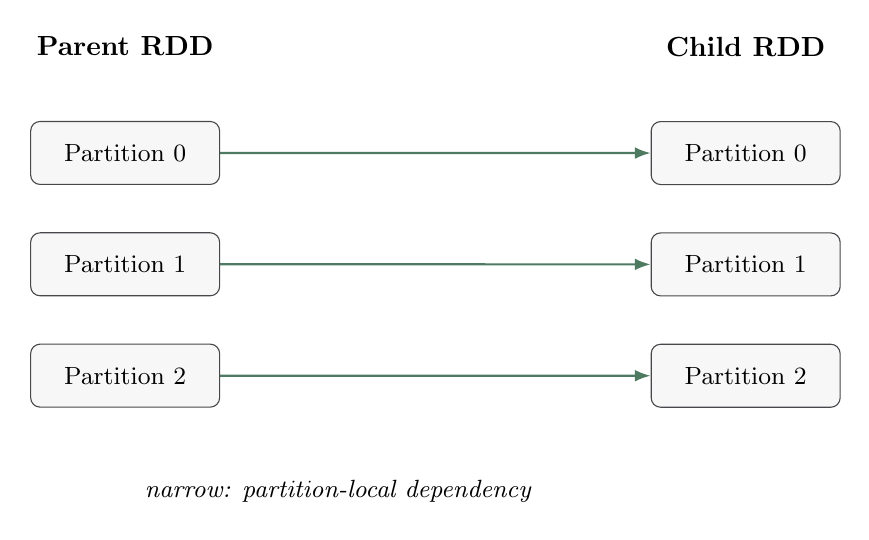
\begin{tikzpicture}[node distance=6mm and 32mm]
\node[font=\bfseries] (ph) {Parent RDD};
\node[font=\bfseries, right=55mm of ph] (ch) {Child RDD};
\node[storagenode, below=7mm of ph] (p0) {Partition 0};
\node[storagenode, below=of p0] (p1) {Partition 1};
\node[storagenode, below=of p1] (p2) {Partition 2};
\node[storagenode, below=7mm of ch] (c0) {Partition 0};
\node[storagenode, below=of c0] (c1) {Partition 1};
\node[storagenode, below=of c1] (c2) {Partition 2};
\draw[-{Latex[length=2mm]},thick,draw=MutedGreen] (p0) -- (c0);
\draw[-{Latex[length=2mm]},thick,draw=MutedGreen] (p1) -- (c1);
\draw[-{Latex[length=2mm]},thick,draw=MutedGreen] (p2) -- (c2);
\node[below=8mm of p2, xshift=27mm, font=\small\itshape] {narrow: partition-local dependency};
\end{tikzpicture}
\caption{Narrow dependency: each child partition can be produced from a corresponding parent partition without network redistribution.}
\label{fig:narrow-dependency}
\end{figure}

\begin{figure}[htbp]
\centering
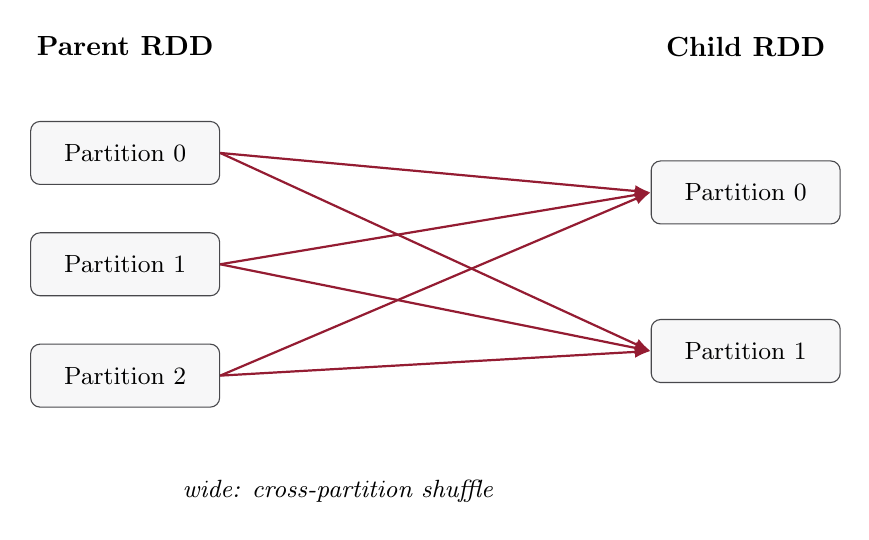
\begin{tikzpicture}[node distance=6mm and 32mm]
\node[font=\bfseries] (ph) {Parent RDD};
\node[font=\bfseries, right=55mm of ph] (ch) {Child RDD};
\node[storagenode, below=7mm of ph] (p0) {Partition 0};
\node[storagenode, below=of p0] (p1) {Partition 1};
\node[storagenode, below=of p1] (p2) {Partition 2};
\node[storagenode, below=12mm of ch] (c0) {Partition 0};
\node[storagenode, below=12mm of c0] (c1) {Partition 1};
\foreach \p in {p0,p1,p2}{
  \draw[shufflearrow] (\p.east) -- (c0.west);
  \draw[shufflearrow] (\p.east) -- (c1.west);
}
\node[below=8mm of p2, xshift=27mm, font=\small\itshape] {wide: cross-partition shuffle};
\end{tikzpicture}
\caption{Wide dependency: each child partition may require records originating from several parent partitions, forcing network redistribution.}
\label{fig:wide-dependency}
\end{figure}

\subsection{Why Dependency Type Determines Stage Boundaries}

The narrow/wide distinction explains the stage concept precisely:

\begin{itemize}
    \item a chain of narrow transformations can be pipelined on each partition inside one stage;
    \item a wide transformation requires a shuffle, so the next stage cannot proceed until the required redistributed data is available.
\end{itemize}

Therefore, a stage is a maximal run of narrow-dependency transformations. Wide dependencies form the boundaries between stages.

\subsection{Worked DAG: Identifying Narrow and Wide Operations}

For the extended word-count chain:

\begin{center}
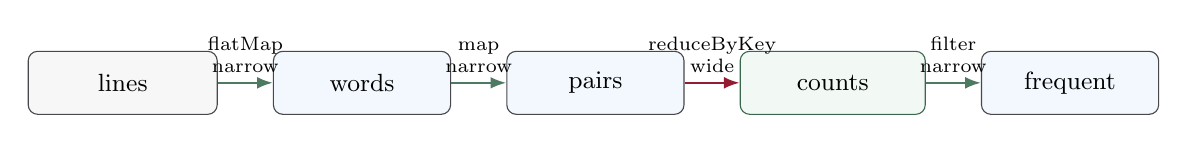
\begin{tikzpicture}[node distance=7mm]
\node[storagenode] (l) {lines};
\node[mapnode, right=of l] (w) {words};
\node[mapnode, right=of w] (p) {pairs};
\node[reducernode, right=of p] (c) {counts};
\node[mapnode, right=of c] (f) {frequent};
\draw[-{Latex[length=2mm]},thick,draw=MutedGreen] (l) -- node[above,font=\scriptsize,align=center]{flatMap\\narrow} (w);
\draw[-{Latex[length=2mm]},thick,draw=MutedGreen] (w) -- node[above,font=\scriptsize,align=center]{map\\narrow} (p);
\draw[shufflearrow] (p) -- node[above,font=\scriptsize,align=center]{reduceByKey\\wide} (c);
\draw[-{Latex[length=2mm]},thick,draw=MutedGreen] (c) -- node[above,font=\scriptsize,align=center]{filter\\narrow} (f);
\end{tikzpicture}
\end{center}

\texttt{flatMap}, \texttt{map}, and \texttt{filter} are narrow. \texttt{reduceByKey} is wide and therefore introduces the shuffle and stage boundary. The five-step logical chain compiles to two physical stages.

\subsection{Performance Implications of Wide Dependencies}

Wide dependencies inherit the same cost characteristics as MapReduce shuffle:

\begin{itemize}
    \item network bandwidth proportional to the volume of redistributed data;
    \item possible disk I/O for shuffle spill and later reads;
    \item a synchronization point because the next stage depends on shuffle output from multiple partitions.
\end{itemize}

Spark does not eliminate shuffle cost. It confines shuffle to the points in the DAG where global redistribution is required.

\subsection{Minimizing Wide Dependencies}

Two practical guidelines follow:

\begin{itemize}
    \item prefer \texttt{reduceByKey} over \texttt{groupByKey} followed by a separate aggregation when local partial aggregation is possible; this is analogous to a MapReduce combiner;
    \item push narrow operations such as filtering before a wide operation when possible, reducing the volume of data that must cross the network.
\end{itemize}

\subsubsection*{Review Questions}
\begin{enumerate}
    \item What distinguishes a narrow dependency from a wide dependency?
    \item Why do narrow dependencies permit pipelining while wide dependencies do not?
    \item Why does the worked word-count chain compile to exactly two physical stages?
    \item How is a wide dependency related to the MapReduce shuffle phase?
\end{enumerate}

% ============================================================
\section{Lineage Tracking and Fault Tolerance}
\label{sec:spark-lineage}
% ============================================================

\subsection{The Fault-Tolerance Problem}

At cluster scale, the failure assumption from the previous chapters remains unchanged: machines holding RDD partitions can fail during computation. The recovery strategies differ by layer:

\begin{itemize}
    \item GFS/HDFS protect stored data through physical replication;
    \item MapReduce re-executes failed tasks from available input;
    \item Spark recomputes specifically lost RDD partitions by following lineage.
\end{itemize}

\subsection{What Lineage Records}

\begin{definitionbox}{Lineage}
Lineage is the recorded chain of transformations that describes how an RDD's partitions were derived from their parent RDD or RDDs. The record includes the parent relationship and the transformation, including the relevant partitioning relationship, used to produce the child.
\end{definitionbox}

The same DAG therefore serves two roles: it is an execution plan before and during normal computation, and it is a recovery plan after data loss.

\subsection{Lineage Stores a Recipe, Not Data Copies}

This is the central difference from distributed-file-system replication. GFS/HDFS retain multiple physical copies of data. Spark can retain a compact derivation description and recreate missing data when required. The lineage metadata is small relative to the intermediate dataset it describes: it stores a compact derivation description rather than another physical copy of the full dataset.

\subsection{How a Lost Partition Is Recomputed}

If a partition disappears, Spark can rebuild exactly the required partition:

\begin{enumerate}
    \item identify the parent partition or partitions recorded in its lineage;
    \item reapply the transformation that produced the missing partition;
    \item if a required parent partition is also missing, continue recursively backward through the lineage until available data is reached.
\end{enumerate}

\begin{figure}[htbp]
\centering
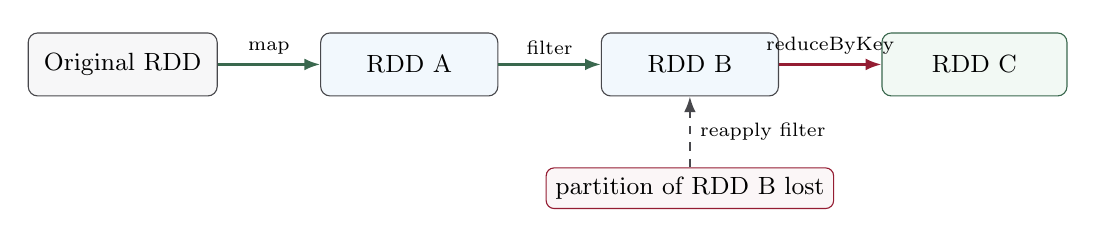
\begin{tikzpicture}[node distance=13mm]
\node[storagenode] (o) {Original RDD};
\node[mapnode, right=of o] (a) {RDD A};
\node[mapnode, right=of a] (b) {RDD B};
\node[reducernode, right=of b] (c) {RDD C};
\draw[datarrow] (o) -- node[above,font=\scriptsize]{map} (a);
\draw[datarrow] (a) -- node[above,font=\scriptsize]{filter} (b);
\draw[shufflearrow] (b) -- node[above,font=\scriptsize]{reduceByKey} (c);
\node[draw=SapienzaRed,rounded corners=1mm,below=9mm of b,fill=SoftRed,font=\small] (lost) {partition of RDD B lost};
\draw[ctrlarrow] (lost) -- node[right,font=\scriptsize]{reapply filter} (b);
\end{tikzpicture}
\caption{Lineage-based recovery. If a partition of RDD B is lost and the required RDD A partition still exists, Spark re-applies the recorded \texttt{filter} only for the missing partition.}
\label{fig:lineage-recompute}
\end{figure}

The important recovery granularity is the partition: unrelated partitions do not need to be recomputed.

\subsection{Comparison with MapReduce Re-Execution}

\begin{table}[htbp]
\centering
\caption{Recovery granularity in MapReduce and Spark.}
\label{tab:mapreduce-spark-recovery}
\begin{tabularx}{\textwidth}{>{\bfseries\raggedright\arraybackslash}p{3.4cm} Y Y}
\toprule
\rowcolor{TableTint}
Aspect & MapReduce & Spark RDDs \\
\midrule
What is recomputed & Failed Map or Reduce task & Specifically lost RDD partition or partitions \\
Recovery granularity & Whole task & Individual partition following lineage \\
Multi-step pipelines & Failure handled within each separate job & One lineage chain can span the complete DAG \\
\bottomrule
\end{tabularx}
\end{table}

Spark therefore generalizes MapReduce's ``recompute the work'' philosophy from a two-stage job to arbitrarily deep RDD transformation graphs.

\subsection{Comparison with GFS/HDFS Replication}

\begin{table}[htbp]
\centering
\caption{Replication-based and lineage-based fault tolerance.}
\label{tab:replication-vs-lineage}
\begin{tabularx}{\textwidth}{>{\bfseries\raggedright\arraybackslash}p{3.6cm} Y Y}
\toprule
\rowcolor{TableTint}
Aspect & GFS/HDFS & Spark RDDs \\
\midrule
Fault-tolerance mechanism & Physical replication of data & Lineage-based recomputation \\
Storage overhead & Multiple physical copies; a typical comparison uses $3\times$ replication & Minimal lineage metadata relative to the data itself \\
Recovery cost & Read an existing replica & Recompute the missing partition; cost can grow when lineage is long \\
\bottomrule
\end{tabularx}
\end{table}

This is a trade-off rather than an unconditional improvement. Replication spends storage continuously to make recovery fast. Lineage minimizes intermediate storage overhead but can make recovery computationally expensive when the derivation chain is deep.

\subsection{Why Replicating Every Intermediate RDD Is Expensive}

A Spark program may generate many intermediate RDDs. Replicating each one would require storing and maintaining multiple physical copies of every intermediate dataset. A ten-transformation pipeline makes the contrast concrete: a replication-based strategy would have to retain ten separate replicated intermediate datasets, while lineage stores a small amount of metadata per RDD.

\subsection{Long Lineage and Checkpointing}

Long lineage chains have a clear weakness. Losing a partition near the end of a deep DAG may require recomputing many preceding steps. Iterative algorithms can make this especially costly because each iteration lengthens the derivation history.

\begin{definitionbox}{Checkpointing}
Checkpointing writes an RDD's current materialized data to durable replicated storage such as HDFS. The checkpoint becomes a new recovery base so future recomputation does not need to traverse the complete earlier lineage chain.
\end{definitionbox}

Checkpointing therefore trades an explicit storage and replication cost now for a bounded recomputation cost later.

\subsection{Recovery Reuses the DAG Scheduler}

Fault recovery is integrated into ordinary scheduling. When a task or worker failure causes partitions to disappear, the DAG scheduler identifies the affected partitions and schedules replacement tasks using the same dependency and stage structure already used for normal execution. Spark does not require a completely separate recovery architecture.

\subsubsection*{Review Questions}
\begin{enumerate}
    \item How does lineage-based fault tolerance differ fundamentally from GFS/HDFS replication?
    \item Walk through how Spark recovers one lost RDD partition.
    \item Why can long lineage chains become a liability, and how does checkpointing address this?
    \item In what sense does Spark reuse its normal DAG machinery for fault recovery?
\end{enumerate}

% ============================================================
\section{Synthesis: From Transformations to Cluster Tasks}
\label{sec:spark-synthesis}
% ============================================================

\subsection{The Full Spark Execution Model}

The mechanisms introduced throughout the chapter form one execution pipeline:

\begin{figure}[htbp]
\centering
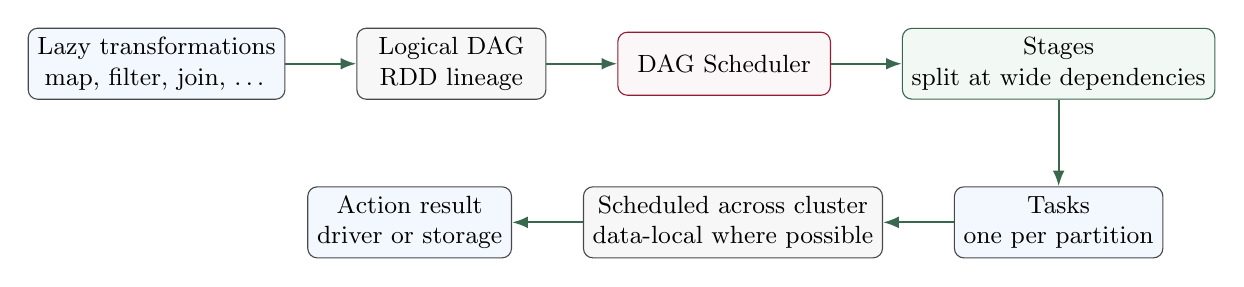
\begin{tikzpicture}[node distance=9mm]
\node[mapnode] (t) {Lazy transformations\\map, filter, join, \ldots};
\node[storagenode, right=of t] (dag) {Logical DAG\\RDD lineage};
\node[masternode, right=of dag] (sched) {DAG Scheduler};
\node[reducernode, right=of sched] (stages) {Stages\\split at wide dependencies};
\node[mapnode, below=11mm of stages] (tasks) {Tasks\\one per partition};
\node[storagenode, left=of tasks] (cluster) {Scheduled across cluster\\data-local where possible};
\node[clientnode, left=of cluster] (action) {Action result\\driver or storage};
\draw[datarrow] (t) -- (dag);
\draw[datarrow] (dag) -- (sched);
\draw[datarrow] (sched) -- (stages);
\draw[datarrow] (stages) -- (tasks);
\draw[datarrow] (tasks) -- (cluster);
\draw[datarrow] (cluster) -- (action);
\end{tikzpicture}
\caption{Spark execution model from lazy transformations to physical tasks. Narrow chains are pipelined within stages, while wide dependencies introduce shuffle boundaries between stages.}
\label{fig:spark-full-execution}
\end{figure}

The action is the trigger. The logical lineage graph already exists before that action; execution converts the required part of the graph into physical stages and tasks.

\subsection{Role of the DAG Scheduler}

The DAG scheduler is Spark's coordinating component, conceptually analogous to the computation coordinator in MapReduce. Once an action is called, it:

\begin{enumerate}
    \item walks the required lineage backward from the action's target RDD;
    \item groups chains of narrow dependencies into pipelined stages;
    \item orders those stages so that each stage's wide-dependency shuffle inputs are available;
    \item creates one task per partition inside each stage and submits those tasks for execution.
\end{enumerate}

\subsection{Data Locality Reappears}

Spark preserves the data-local scheduling principle from the earlier chapters. For an initial stage reading from HDFS/GFS, tasks are preferably placed on machines holding the corresponding storage blocks. For later stages, the scheduler prefers machines where required cached parent partitions already reside in memory whenever possible.

\begin{keyconcept}
The same ``move computation to data'' principle appears at three layers of the course: distributed storage exposes block placement, MapReduce schedules Map tasks near those blocks, and Spark additionally tries to schedule later work near already materialized or cached RDD partitions.
\end{keyconcept}

\subsection{Strengths of the Spark/RDD Model}

Relative to the MapReduce model developed in Chapter~2, four strengths stand out:

\begin{itemize}
    \item \textbf{Generality:} arbitrary DAGs replace a fixed two-stage shape.
    \item \textbf{Performance for iterative and interactive workloads:} in-memory caching avoids repeated disk round-trips.
    \item \textbf{Efficient fault tolerance:} lineage avoids full physical replication of every intermediate dataset.
    \item \textbf{Optimizable execution:} visibility of the full logical pipeline enables pipelining and avoidance of unnecessary materialization.
\end{itemize}

\subsection{Remaining Limitations}

The original RDD model still has limitations:

\begin{itemize}
    \item the RDD API is relatively low-level for complex relational-style queries;
    \item RDDs do not inherently expose schema and column semantics that could enable richer structured-data optimization;
    \item the original model is batch-oriented and does not by itself represent continuous, unbounded streaming data.
\end{itemize}

\subsection{Beyond the Original RDD Model}

Several modern systems extend the broader design space:

\begin{itemize}
    \item \textbf{Apache Flink:} continuous processing of unbounded streams;
    \item \textbf{Ray:} dynamic distributed task graphs for AI workloads;
    \item \textbf{Delta Lake:} a unified lakehouse storage abstraction connecting data-lake storage with structured tables.
\end{itemize}

These examples do not replace the RDD model developed here; they illustrate how modern infrastructure extends the design space beyond the original batch-oriented abstraction.

% ============================================================
\section{Key Terms}
% ============================================================

\begin{table}[htbp]
\centering
\caption{Key Spark terminology.}
\label{tab:spark-key-terms}
\begin{tabularx}{\textwidth}{>{\bfseries\raggedright\arraybackslash}p{3.4cm} Y}
\toprule
\rowcolor{TableTint}
Term & Meaning \\
\midrule
RDD & Immutable, partitioned, distributed dataset with tracked lineage. \\
Transformation & Lazy operation that produces a new RDD, such as \texttt{map} or \texttt{filter}. \\
Action & Operation that triggers execution and returns or writes a result. \\
Narrow dependency & Child partition depends on a small fixed number of parent partitions; permits pipelining. \\
Wide dependency & Child partition depends on multiple parent partitions; requires a shuffle. \\
Lineage & Recorded transformation history that enables recomputation. \\
Stage & Maximal pipelinable group of operations between shuffle boundaries. \\
Checkpoint & Durable materialization used to bound the cost of recomputing a long lineage chain. \\
DAG scheduler & Component that derives stages and tasks from the logical lineage graph after an action triggers execution. \\
\bottomrule
\end{tabularx}
\end{table}

% ============================================================
\section{Chapter Summary}
% ============================================================

\begin{longtable}{>{\bfseries\raggedright\arraybackslash}p{\dimexpr0.23\textwidth-2\tabcolsep\relax} >{\raggedright\arraybackslash}p{\dimexpr0.34\textwidth-2\tabcolsep\relax} >{\raggedright\arraybackslash}p{\dimexpr0.43\textwidth-2\tabcolsep\relax}}
\caption{Compact summary of the Spark/RDD execution model.}
\label{tab:spark-core-summary}\\
\toprule
Concept & Main role & Key relationship / trade-off \\
\midrule
\endfirsthead
\toprule
Concept & Main role & Key relationship / trade-off \\
\midrule
\endhead
RDD & Distributed immutable dataset abstraction & Partitioned for parallelism and described by lineage. \\
Transformation & Build a derived RDD lazily & Extends the DAG without immediately executing data processing. \\
Action & Trigger computation & Converts the required logical plan into physical execution. \\
Caching & Reuse computed partitions & Improves iterative and interactive performance but consumes memory or persistence capacity. \\
Logical DAG & Record dependencies & Gives Spark whole-pipeline visibility before execution. \\
Narrow dependency & Partition-local relationship & Enables pipelining inside one stage. \\
Wide dependency & Cross-partition relationship & Forces shuffle and creates a stage boundary. \\
Stage & Pipelined physical segment & Maximal sequence of operations not separated by a shuffle. \\
Task & Per-partition unit of execution & Stage parallelism is realized through tasks distributed across workers. \\
Lineage & Recovery recipe & Avoids replicating every intermediate RDD but can make recovery expensive when chains are long. \\
Checkpointing & Bound lineage depth & Pays durable-storage cost to reduce future recomputation cost. \\
DAG scheduler & Coordinate execution & Converts dependencies into ordered stages and tasks and reuses the same structure for recovery. \\
Data locality & Place work near needed data & Extends the locality principle from DFS blocks to cached RDD partitions. \\
\bottomrule
\end{longtable}

% ============================================================
\section{Quick Review}
% ============================================================

\begin{enumerate}
    \item Spark was designed to address the disk-heavy, rigid, high-latency limitations of chained MapReduce jobs.
    \item A Spark computation is represented as an arbitrary DAG rather than a fixed two-stage pipeline.
    \item Memory-centric execution is especially useful when the same working dataset is reused across iterations or interactive queries.
    \item An RDD is immutable, partitioned, distributed, and lineage-tracked.
    \item RDD partitions are computation-level units and are related to, but not identical with, distributed-storage blocks.
    \item \texttt{textFile} can build an RDD from distributed storage; \texttt{parallelize} can distribute a driver-side collection.
    \item An RDD can exist as a logical description before its contents are materialized.
    \item Caching retains computed partitions for fast reuse; persistence can use memory, disk, or a mixture.
    \item Transformations create new RDD descriptions and are lazy.
    \item Actions trigger the computation needed to return or write a result.
    \item Lazy evaluation gives Spark visibility over the complete transformation chain before execution.
    \item Compatible narrow transformations can be pipelined in one pass without full intermediate materialization.
    \item A logical DAG is divided into stages when execution is triggered.
    \item Narrow dependencies keep computation partition-local and therefore permit pipelining.
    \item Wide dependencies require cross-partition redistribution and therefore cause shuffle.
    \item Stage boundaries coincide with wide-dependency boundaries.
    \item Spark does not eliminate shuffle; it limits shuffle to the points where redistribution is required by the DAG.
    \item \texttt{reduceByKey} can reduce shuffle volume through local partial aggregation compared with grouping all values first.
    \item Lineage records how RDD partitions were derived from parent RDDs.
    \item If a partition is lost, Spark recomputes that partition by walking backward through lineage to available data.
    \item Lineage avoids the storage cost of replicating every intermediate RDD, but recovery cost grows with lineage depth.
    \item Checkpointing writes an RDD to durable replicated storage and resets the effective recovery base.
    \item The DAG scheduler groups narrow chains into stages and creates one task per partition inside each stage.
    \item Spark's scheduler preserves data locality both for initial DFS input and for later cached partitions when possible.
    \item The original RDD model remains relatively low-level for structured relational queries and does not by itself model unbounded streaming data.
\end{enumerate}

% ============================================================
\section{Further Reading}
% ============================================================

Further reading includes:

\begin{itemize}
    \item Zaharia, M., et al. (2012). \emph{Resilient Distributed Datasets: A Fault-Tolerant Abstraction for In-Memory Cluster Computing}. NSDI.
    \item Course reference materials on Spark execution internals.
\end{itemize}



\backmatter
\chapter*{Combined Quick Reference}
\addcontentsline{toc}{chapter}{Combined Quick Reference}
\markboth{Combined Quick Reference}{Combined Quick Reference}

The first three chapters form one continuous scale-out stack. Distributed storage provides durable, location-aware blocks. MapReduce turns those blocks into data-local batch tasks connected by shuffle. Spark generalizes the computation layer into a lazy DAG, retains reusable partitions in memory when possible, and recovers lost intermediate state through lineage-based recomputation.

\begin{table}[htbp]
\centering
\small
\caption{Distributed storage, MapReduce, and Spark viewed as one scale-out architecture.}
\begin{tabularx}{\textwidth}{>{\bfseries\raggedright\arraybackslash}p{2.55cm} Y Y Y}
\toprule
\rowcolor{TableTint}
Concern & Distributed storage & MapReduce & Spark / RDDs \\
\midrule
Basic unit & Block / chunk & Map or Reduce task & RDD partition / task \\
Coordinator & Master / NameNode & Master / JobTracker & DAG scheduler \\
Execution shape & Storage namespace and replica graph & Fixed Map $\rightarrow$ Shuffle $\rightarrow$ Reduce job & Arbitrary lazy DAG split into stages \\
Placement goal & Durable replicas across failure domains & Data-local Map execution & Data-local tasks and reuse of cached partitions \\
Failure detection & Heartbeats, block reports, checksums & Worker heartbeats and progress tracking & Task/worker failure handled through scheduler state \\
Recovery & Re-replication & Re-execution of failed tasks & Lineage-based recomputation of lost partitions \\
Network-sensitive operation & Cross-rack replication & Shuffle & Wide-dependency shuffle \\
Intermediate state & Durable replicated blocks & Local Map output plus job-boundary materialization & In-memory partitions when possible; checkpoint when needed \\
Main optimization & Placement and direct data transfer & Locality, combiners, speculation & Laziness, pipelining, caching, stage optimization \\
\bottomrule
\end{tabularx}
\end{table}

\end{document}
